\documentclass{article}
%导包
\usepackage{graphicx}
\usepackage{caption}
\usepackage{url}
\usepackage{enumitem}
\usepackage{mathtools}
\usepackage{abstract}
\usepackage{geometry}
\usepackage{lettrine}
\usepackage{multicol}
\usepackage{indentfirst}
\usepackage{cite}
\usepackage{graphics}
\usepackage{subfigure}
\usepackage{booktabs}
\usepackage{multirow}
\usepackage{diagbox}
\usepackage{makecell}
\usepackage{amsthm,amsmath,amssymb}
\usepackage{mathrsfs}
\usepackage{verbatim}
\usepackage{pifont}
\usepackage{amsfonts}
\usepackage{float}
\usepackage[section]{placeins}
\usepackage{wrapfig}
%提前配置的定理环境

%wrj的
\geometry{left=2.0cm, right=2.0cm, top=2.0cm, bottom=2.0cm}
\setlength{\absleftindent}{0pt}
\setlength{\absrightindent}{0pt}
\usepackage[colorlinks,
            linkcolor=black,
             anchorcolor=blue,
             urlcolor=blue,
             citecolor=red]{hyperref}
\newtheorem{Thm}{Theorem}[section]
\newtheorem{Col}[Thm]{Corollary}
\newtheorem{Exe}[subsubsection]{Exercise}
\newtheorem{Ex}{Example}[section]
\newtheorem{Def}{Definition}[section]
\newtheorem{Rk}{Remark}[section]
\newtheorem*{Rk*}{Remark}
\newtheorem{lem}{Lemma}[section]
\newtheorem*{Thm*}{Theorem}
%图片路径以及标题
\graphicspath{{picture/}}
\begin{document}
%正文======================
\title{TRIANGLE GROUP}
\author{Renjing.Wang, Zhenpeng.Liu, Guanyi.Wu, Shihao.Li}
\maketitle

\section{Background and Introduction}%背景,抄一抄题目
Tesselation has many applications in several fields incluidng arts, architecture and also geometry itself. A tessellation or tiling is the covering of a surface, often a plane, using one or more geometric shapes, called tiles, with no overlaps and no gaps. Naturally, we have different patterns of tiling such as periodic tiling which can be catagorized into 17 wallpaper groups and aperidodic tiling. However, in this report, we mainly consider the triangle tiling of the plane using only reflection but with  different groups of triangles (known as Euclidean triangle, Sphereical triangle and Hyperbolic triangle).

If you begin with a Euclidean triangle, then reflect across one of its sides, you obtain another copy of the triangle. If you keep repeating this process, is it possible to tile the Euclidean plane, where no two triangles overlap? This process certainly works for equilateral triangles, but we cannot expect this to work in general. In fact, there are only 3 triangular shapes that work for the Euclidean plane. However, we can also consider this question for spherical triangles or hyperbolic triangles.

\section{General (p, q, r) Triangle Group}
Instead of defining all the things in terms of languages in abstract algebra, an easy example will be firstly demostrated to get into the topic.
\begin{Ex}
    Let's firstly consider a ``fundamental" isosceles right triangle in the Euclidean plane, such as the one outlined in the pattern in Figure \ref{2-4-4}. Let $x$ and $y$ be reflections about the lines along the legs of the triangle, and let $z$ be reflection about the line along the hypotenuse.
    Intuitively speaking, Euclidean plane will be tiled without overlapping if we proceed our instruction countably many times. And as Figure \ref {2-4-4} indicated, half the triangles in the pattern have the same orientation as the fundamental triangle and half the opposite, and you can tell through the forward and backward Fs.
\end{Ex}
\begin{figure}[ht]
    \includegraphics[width = 0.5\linewidth]{"2-4-4"}
    \centering
    \caption{The full (2,4,4) triangle group}
    \label{2-4-4}
\end{figure}
This construction certain applies to other triangles.
And it's not hard to see that each angle $\alpha$ of the
fundamnetal triangle should be of the form $2\pi/p$,
where p is a positive integer. Because otherwise consider
a triangle with $p$ a non-integer, let's say a triangle with
degree $107^{\circ}$. It's clearly that after 3-times reflection,
there is still an empty corner and if we do another reflection,
it will overlap the previous pattern. (See Figure \ref{107}.)

But is the form $2\pi/p$ enough? The answer is YES if we don't
consider the orientation. But in our context, orientation is always
taken into account so the answer should be NO. To illustate this,
let's consider an isosceles triangle with the top angle equal to $120^{\circ}$.
Clearly if we change the order of compositions of reflections,
the orientation of the fundamnetal triangle will be different.
Although this will not influence the tesselation of the whole plane,
that's not what we want. Therefore, we also have to ask each angle
to be the form $\pi/p$, where $p$ is a positive integer.(See Figure \ref{120}.)
\begin{figure}[htbp]
    \begin{minipage}{0.32\linewidth}
        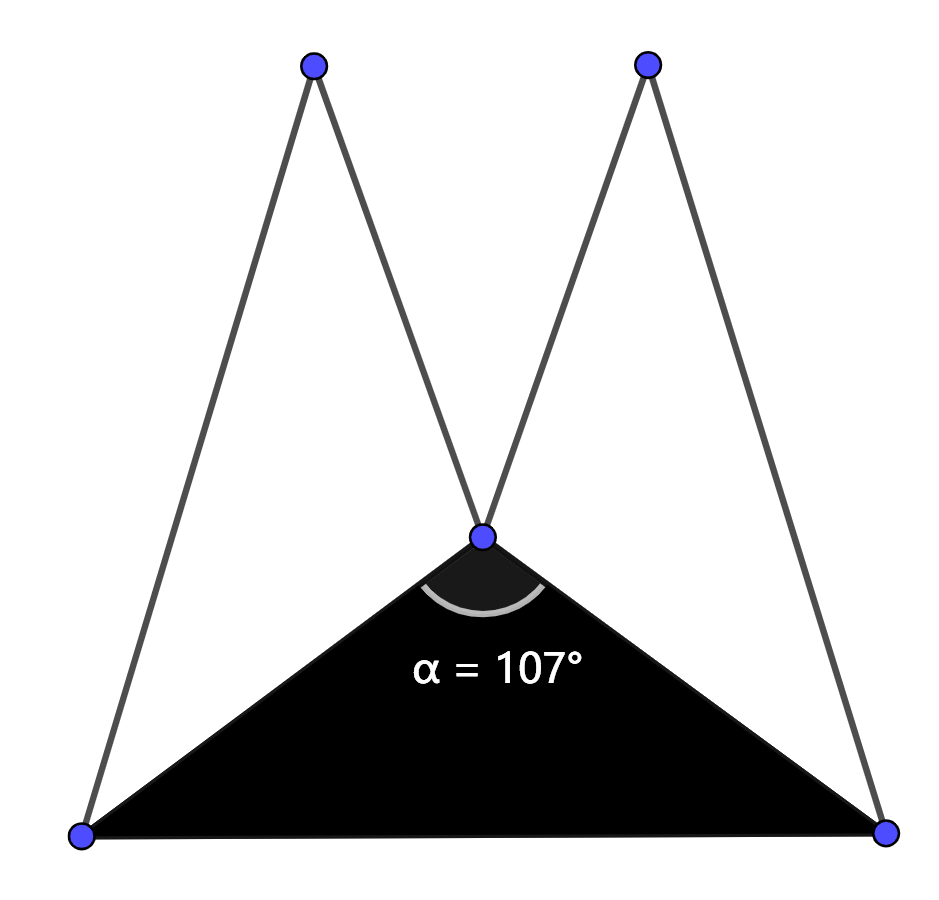
\includegraphics[width={0.9\linewidth}]{107.png}
        \centering
        \caption{Triangles with one angle equal $107^{\circ}$}
        \label{107}
    \end{minipage}
    \begin{minipage}{0.65\linewidth}
        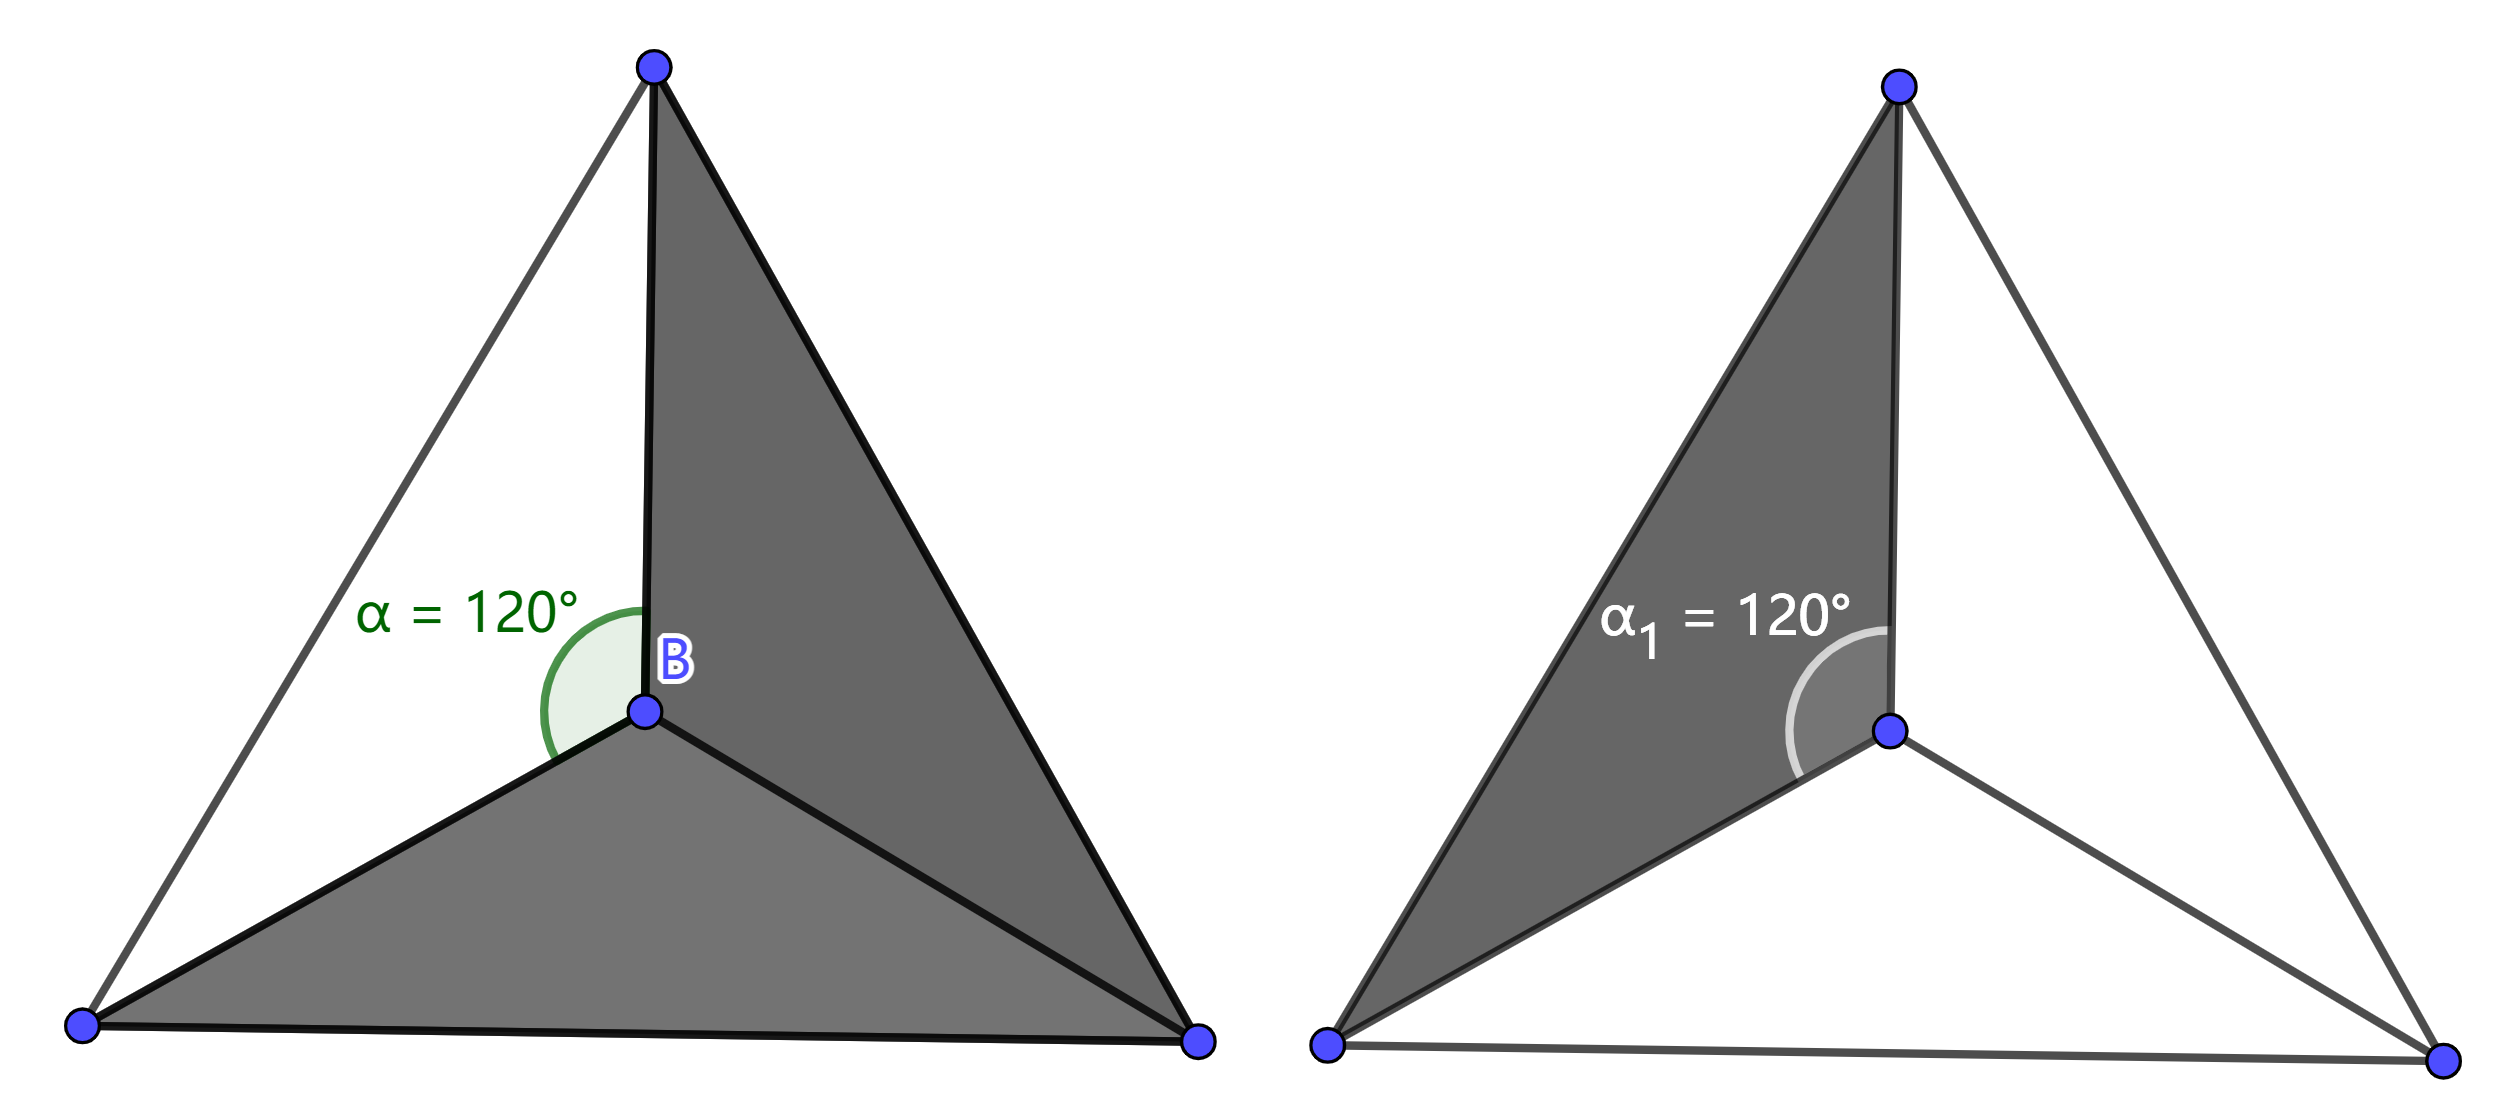
\includegraphics[width={0.9\linewidth}]{120.png}
        \centering
        \caption{Triangles with one angle equal $120^{\circ}$}
        \label{120}
    \end{minipage}
\end{figure}
We are now ready to define a $(p, q, r)$ triangle.
\begin{Def}
    A $\textbf{(p, q, r)}$ \textbf{triangle} is one with angles $\pi/p, \pi/q, \pi/r$, where $p$, $q$, $r$ are positive integers.
\end{Def}
\begin{Def}
    Let $p, q, r$ be the positive integers $\geq 2$ and define $\lambda$ to be
    $$
        \lambda=\frac{1}{p}+\frac{1}{q}+\frac{1}{r}-1
    $$
    So, a full triangle group  is reflection roup which is generated by the reflections of all sides of the triangle with angles $\frac{\pi}{p}, \frac{\pi}{q}, \frac{\pi}{r}$.

    Now if
    \item $\lambda>0$ then $\Delta$ is Spherical,
    \item $\lambda<0$ then $\Delta$ is Hyperbolic,
    \item $\lambda=0$ then $\Delta$ is Euclidean.
\end{Def}
\begin{Def}
    Given any $(p, q, r)$ triangle, the group of isometries, either Euclidean or spherical or hyperbolic, generated by reflections $x, y, z$ in the three sides of the triangle is called the \textbf{full} \textbf{$\textbf{(p, q, r)}$ triangle group}, and it's denoted by $\Delta(p, q, r)$.
\end{Def}
The symmetry group of Figure \ref{2-4-4} is the full $(2,4,4)$ triangle group.
\begin{Rk}
    The number of elements of a triangle group equals the number of copies of the original triangle in the pattern, because there is a unique isometry in the group taking the fundamental triangle to any other triangle (isometries are determined by what they do to a single triangle and no isometry in the group takes the fundamental triangle to itself, other than the identity).
\end{Rk}
A presentation in terms of generators and relations for the full triangle group $(p, q, r)$ is not difficult to obtain. The three generating reflections $x, y$, and $z$ clearly have order 2 . The product of two reflections in lines meeting at an angle $\alpha$ is a rotation by $2 \alpha$ about the intersection of the two lines. Thus $x y$, $y z$, and $x z$ are rotations by $2 \pi / p, 2 \pi / q$, and $2 \pi / r$ and hence have orders $p$, $q$, and $r$. So far, we have
$$
    x^2=y^2=z^2=1,(x y)^p=(y z)^q=(x z)^r=1
$$
And it turns out that these are only relators needed. The proof is a little bit involved and we just simply omit here. The proof can be seen in \cite{Tgt}.

Given a full $(p, q, r)$ triangle group $\Delta(p, q, r)$, the subgroup $\Delta'(p, q, r)$ generated by the rotations $x y, y z$, and $x z$ at the three vertices of the fundamental triangle is called the ``ordinary" $(p, q, r)$ triangle group. Since $(x y)(y z)=x y^2 z=x z$, this group is generated by $u=x y$ and $v=y z$ alone. It has the presentation
$$
    \left\langle u, v: u^p=v^q=(u v)^r=1\right\rangle
$$
\begin{Thm}
    A full $(p, q, r)$ triangle group $\Delta(p, q, r)$ has the presentation
    $$
        \left\langle x, y, z: x^2=y^2=z^2=1,(x y)^p=(y z)^q=(x z)^r=1\right\rangle
    $$
    Its orientation-preserving subgroup $\Delta'(p, q, r)$ is the ordinary triangle group generated by the rotations u=xy,v=yz and has the presentation
    $$\left\langle u,v:u^p=v^q=(uv)^r=1\right\rangle$$

\end{Thm}
Let's consider the Euclidean, Spherical and Hyperbolic cases respectively.
\section{Classification}
\subsection{Euclidean Triangle Group}
This is the case when $$\frac{1}{p}+\frac{1}{q}+\frac{1}{r}=1$$
Due to the restriction that $p$, $q$, $r$ are all integers, the cases in Euclidean space are just finite. And the knowledge from basic number theory implies the following theorem.
\begin{lem}
    $\triangle(p, q, r)$ is isomorphic to $\triangle(q, r, p)$ i.e. $\triangle(p, q, r) \cong \triangle(q, r, p)$
\end{lem}
\begin{proof}
    We have,
    $$
        \begin{gathered}
            \Delta(p, q, r)=\left\{a, b, c \mid a^2=b^2=c^2=(a b)^r=(b c)^p=(c a)^q=1\right\} \\
            \Delta(m, n, l)=\left\{x, y, z \mid x^2=y^2=z^2=(x y)^p=(y z)^q=(z x)^r=1\right\}
        \end{gathered}
    $$
    Define a map,
    $$
        \phi: \triangle(p, q, r) \rightarrow \triangle(q, r, p)
    $$
    such that
    $$
        \begin{aligned}
             & a \mapsto x \\
             & b \mapsto y \\
             & c \mapsto z
        \end{aligned}
    $$
    let $u, w \in \triangle(p, q, r)$. So we can take $u=a^i b^j c^k$ and $w=a^l b^m c^n$. It can be easily shown that
    $$
        \begin{aligned}
            \phi(u w) =\phi(u) \phi(w)
        \end{aligned}
    $$
    So $\phi$ is a homomorphism. $\phi$ is also surjective and injective. Hence $\phi$ is isomorphism. Therefore $\triangle(p, q, r)$ and $\triangle(p, q, r)$ is isomorphic.
\end{proof}
\begin{Thm}
    Only values of the triple $(p, q, r)$ can take in Euclidean plane are: $(2,3,6),(2,4,4)$ and $(3,3,3)$.
\end{Thm}
\begin{proof}
    It's easy to see by basic number theory and the above lemma.
\end{proof}
\subsubsection{Nice pictures of Euclidean triangle tiling}
Nice pictures of triangle tesselation in Euclidean plane are listed as follows:
\begin{figure}[h]%给一些图片的例子
    \centering
    \begin{minipage}{0.22\linewidth}
        \centering
        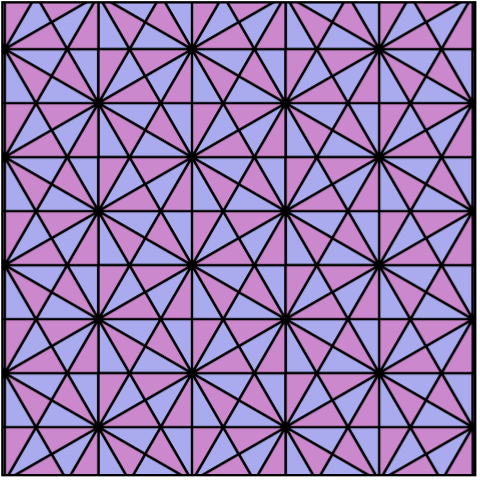
\includegraphics[width={0.8\linewidth}]{2_3_6.png}
        \caption{(2,3,6)}
    \end{minipage}
    \begin{minipage}{0.22\linewidth}
        \centering
        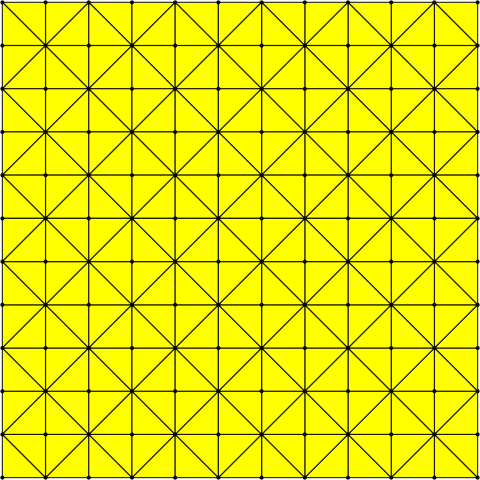
\includegraphics[width={0.8\linewidth}]{2_4_4.png}
        \caption{(2,4,4)}
    \end{minipage}
    \begin{minipage}{0.22\linewidth}
        \centering
        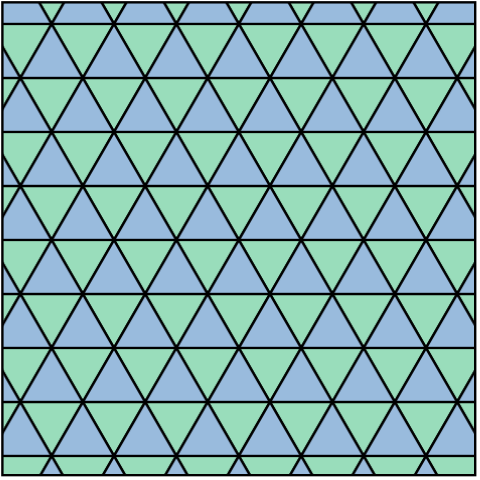
\includegraphics[width={0.8\linewidth}]{3_3_3.png}
        \caption{(3,3,3)}
    \end{minipage}
\end{figure}
%=================================WGY===================
\subsection{Spherical Triangle Group}
As demonstrated in the Euclidean plane, there are only some special cases for spherical triangles. And we summarzie the results in the following theorem.
\begin{Thm}
    Only possibilities of the triple (p, q, r) can take in Spherical case are:
    $$(2,3,3), (2,3,4), (2,3,5)\hspace{1mm} or \hspace{1mm}(2,2,n)_{n>1}$$
\end{Thm}

\begin{Rk*}
    Here we do not include the case when $n=1$ which is a degenerated case.
\end{Rk*}

Different from Euclidean plane tesselation, only finite reflections are needed for spherical case becasue the area of a sphere is always finite. And the exact times of reflection can be computed due to the fact that the area for a spherical triangle with inner angles $\alpha$, $\beta$, $\gamma$ is ($\alpha + \beta + \gamma - \pi)r$, where r is the radius of the sphere. Let's consider the following example.
\begin{Ex}
    Consider using the spherical triangle A:(2,3,3) to tile the spherical plane.
    The area of A is: $$S_A = (\pi/2+\pi/3+\pi/3-\pi)r^2=\pi r^2/6$$
    The total area of the surface is : $$S= 4\pi r^2$$
    Hence the times of reflection is: $$n=\frac{ 4\pi r^2}{\pi r^2/6}=24.$$
    The tiling picture is depicted in Figure \ref{fig:subim9}.
\end{Ex}

Also, we can see the spherical triangle in another perspective which will help us gain more insight.
Actually, spherical triangle groups can be identified with the symmetry groups of regular polyhedra in the three-dimensional Euclidean space: $\Delta(2,3,3)$ corresponds to the tetrahedron, $\Delta(2,3,4)$ to both the cube and the octahedron (which have the same symmetry group), $\Delta(2,3,5)$ to both the dodecahedron and the icosahedron. Then, the spherical tiling corresponding to a regular polyhedron is obtained by forming the barycentric subdivision of the polyhedron and projecting the resulting points and lines onto the circumscribed sphere. Let me demonstrate this in the following example.
\begin{Ex}
    In the case of the tetrahedron, there are four faces and each face is an equilateral triangle that is subdivided into 6 smaller pieces by the medians intersecting in the center. The resulting tesselation has 4 × 6=24 spherical triangles. That's the same number as we obtained in the previous $(2, 3, 3)$ case! See Figure \ref{tetrahedron}.
\end{Ex}
%\begin{figure}[h]
%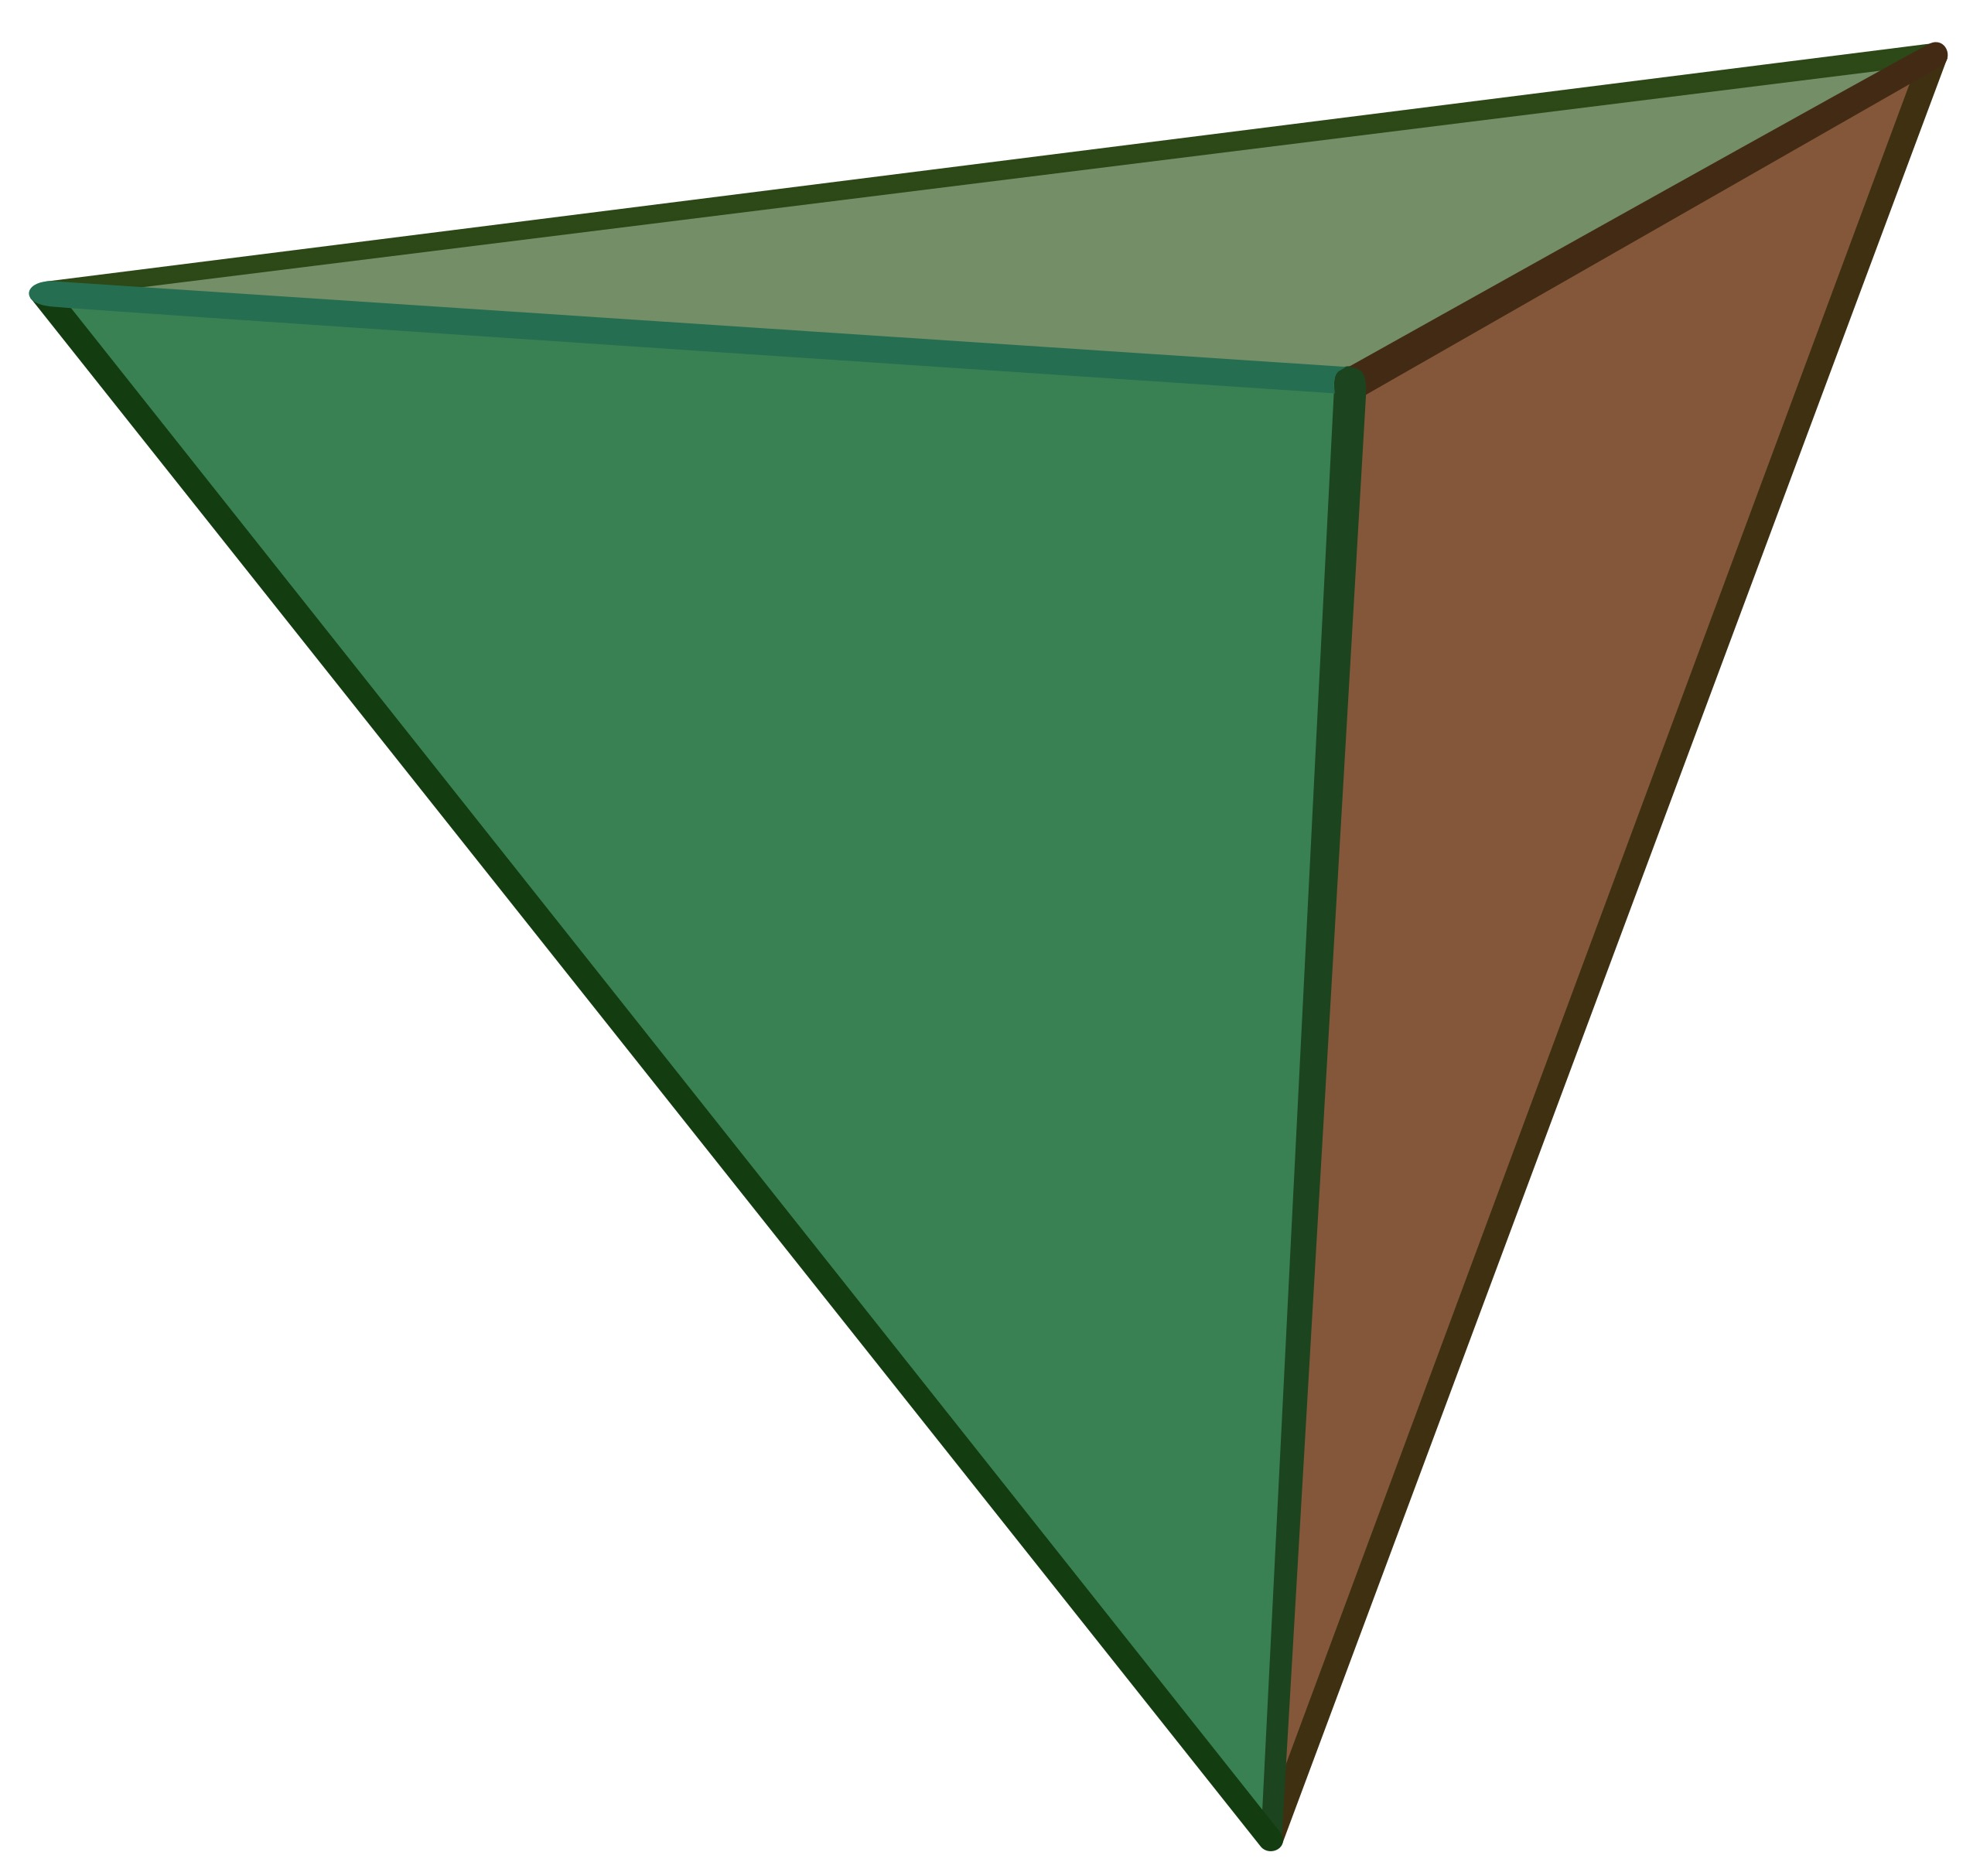
\includegraphics[scale=0.04]{tetrahedron.jpg}
%\centering
%\caption{tetrahedron}
%\label{tetrahedron}
%\end{figure}

\begin{figure}[ht]
    \centering
    \begin{minipage}{0.32\linewidth}
        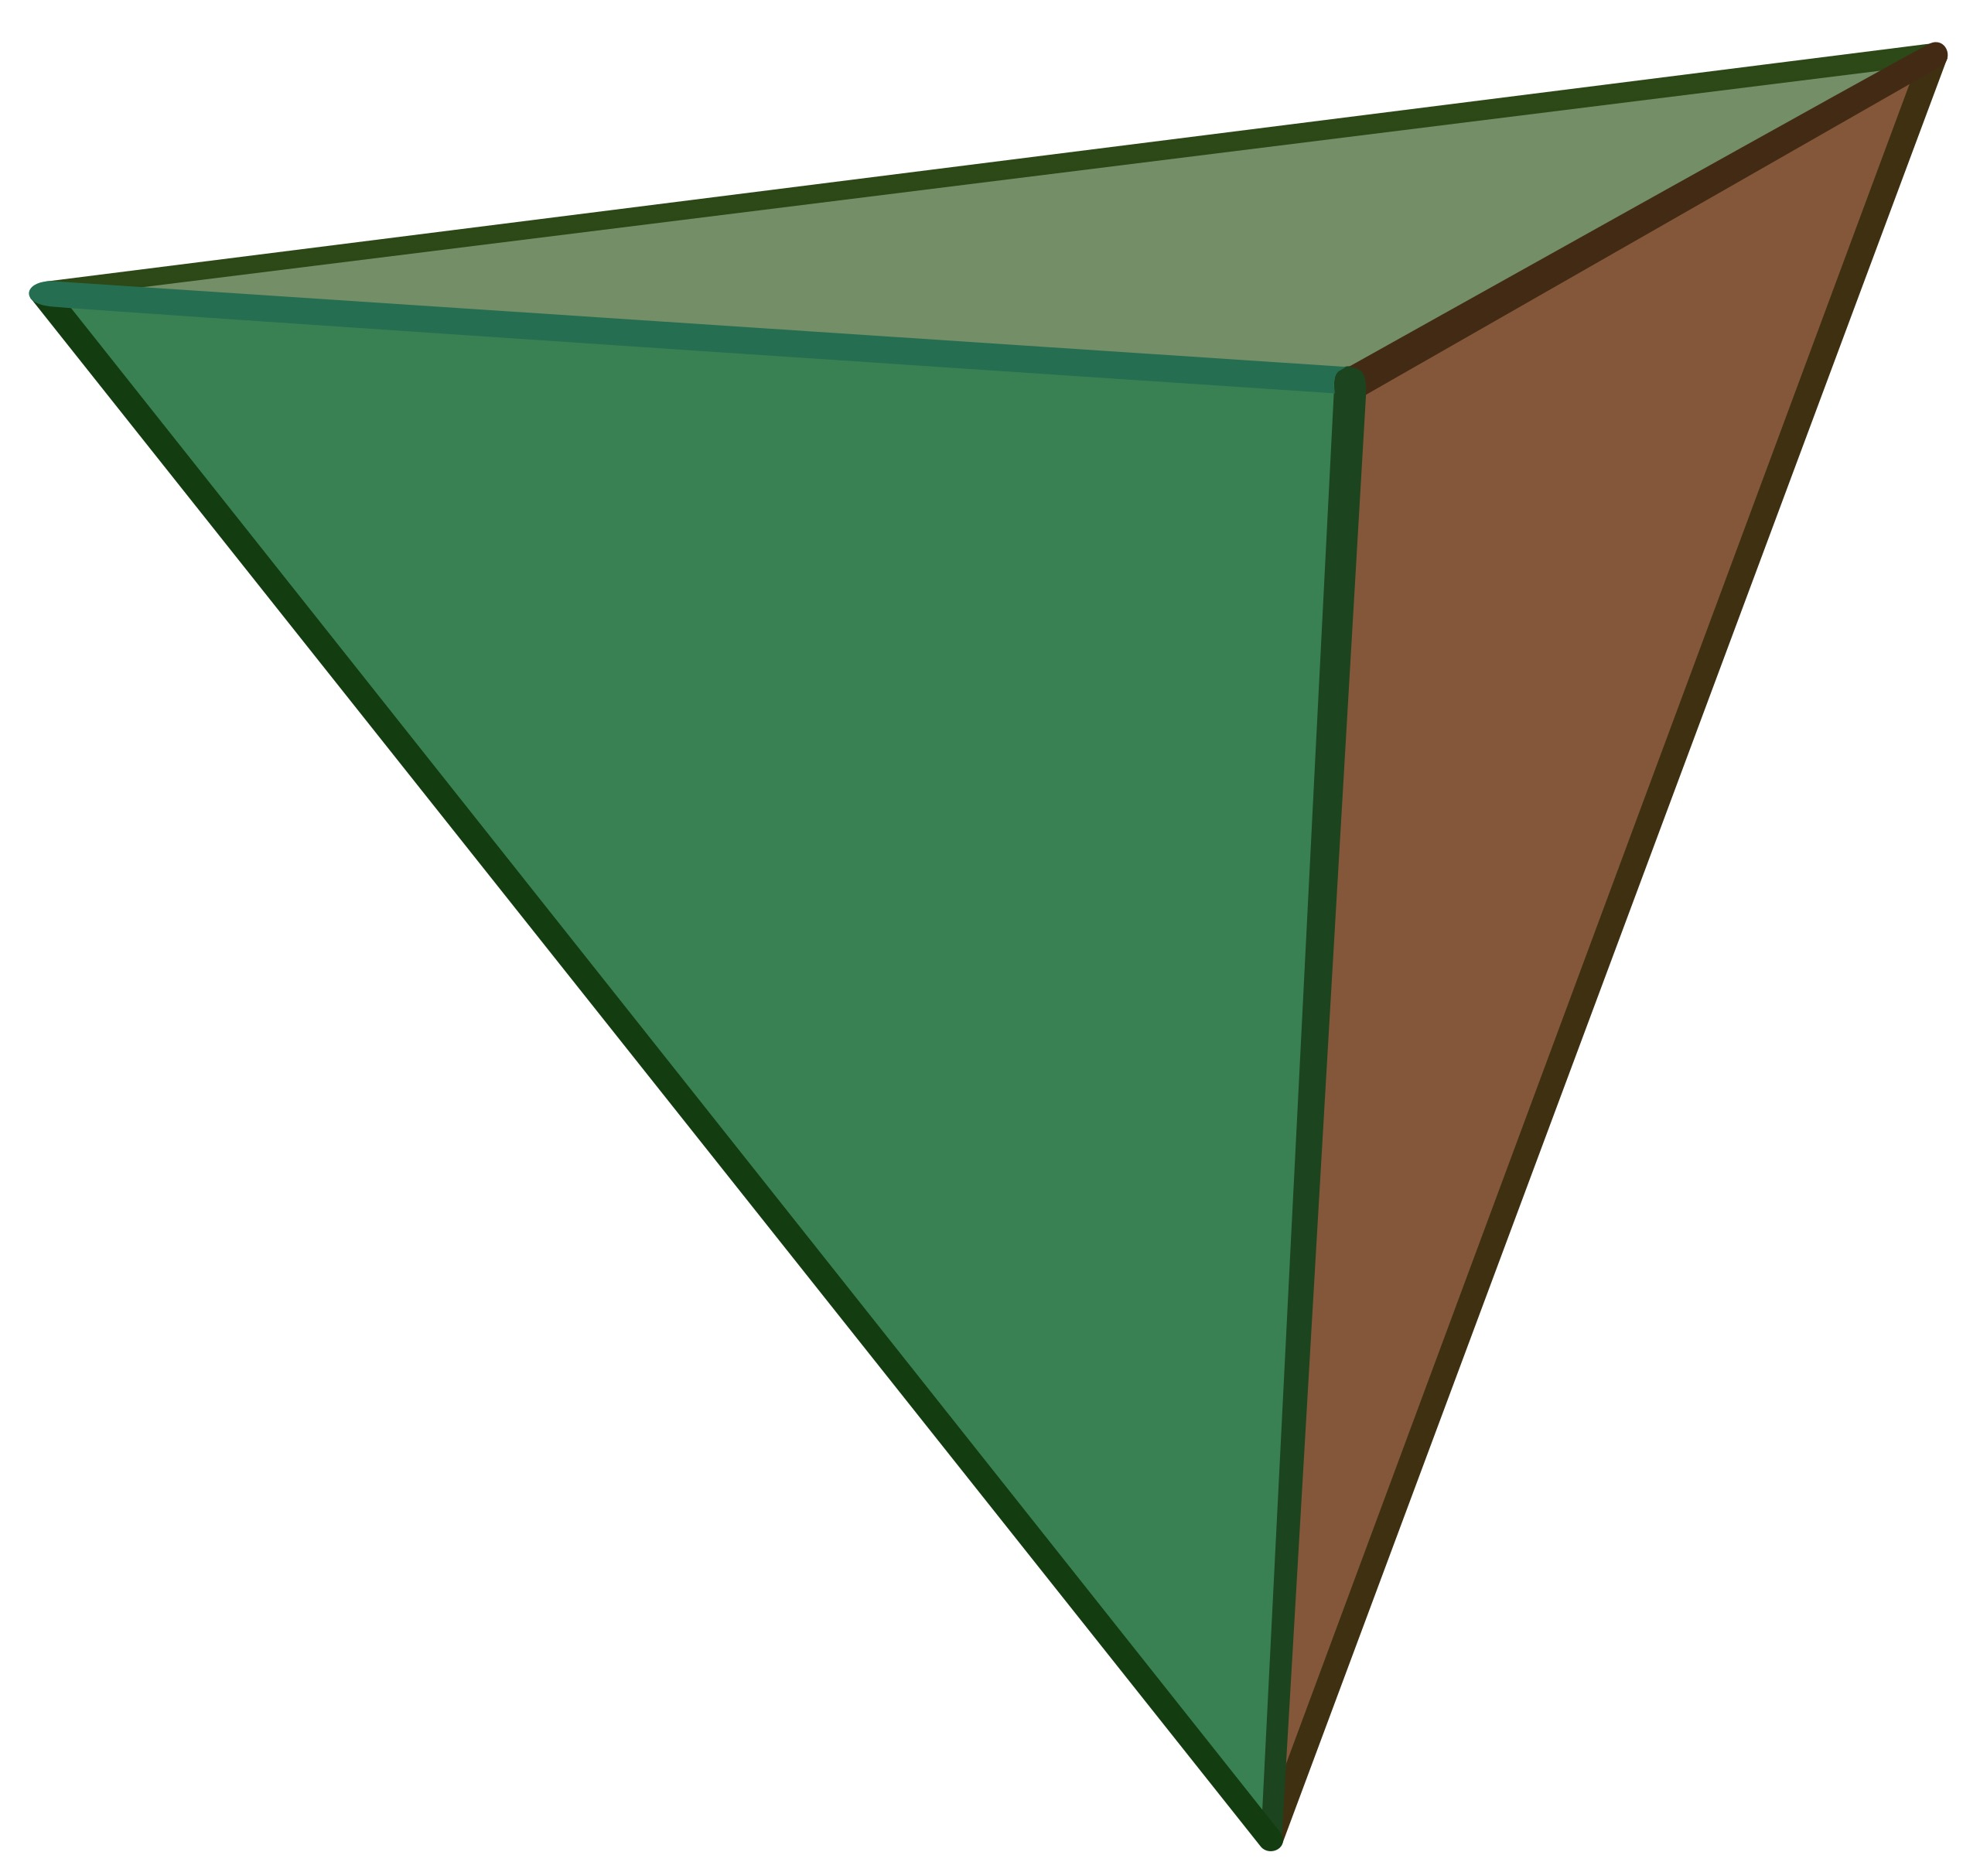
\includegraphics[width=0.9\linewidth]{tetrahedron.jpg}
        \caption{tetrahedron}
        \label{tetrahedron}
    \end{minipage}
    \begin{minipage}{0.32\linewidth}
        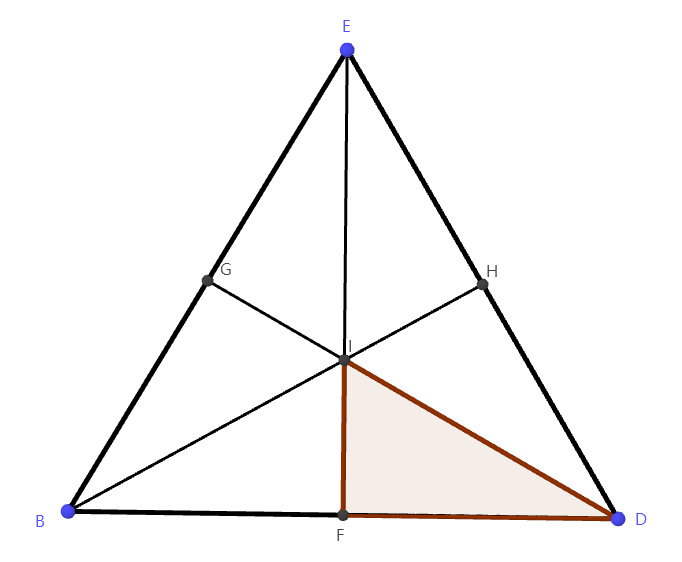
\includegraphics[width=0.9\linewidth]{spheretri.png}
        \caption{spheretri}
        \label{sphere_tri}
    \end{minipage}
    \begin{minipage}{0.32\linewidth}
        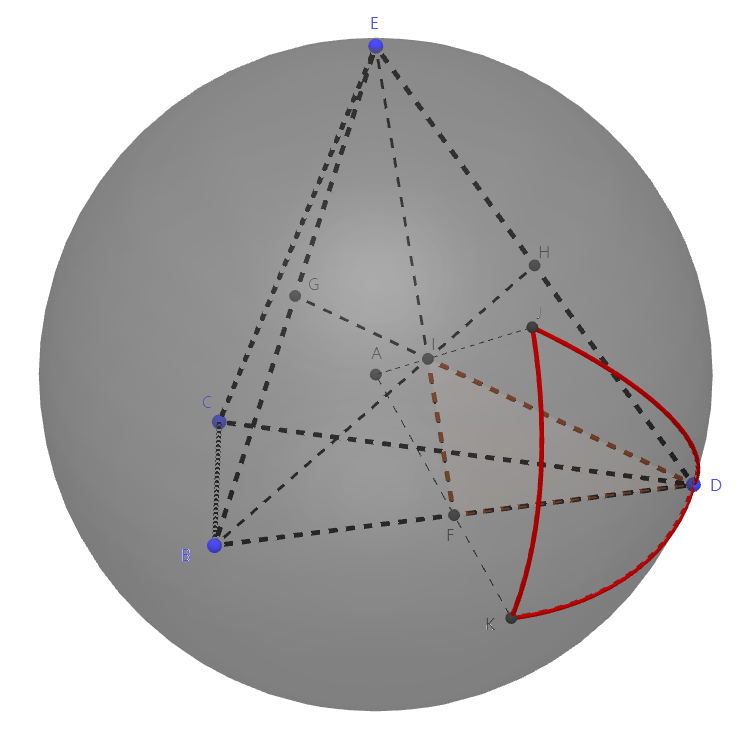
\includegraphics[width=0.9\linewidth]{sphere.png}
        \caption{sphere}
        \label{sphere}
    \end{minipage}
\end{figure}

\newpage
\subsubsection{Nice pictures of Spherical triangle tiling}
\begin{figure}[ht]
    \centering
    \begin{minipage}{0.2\linewidth}
        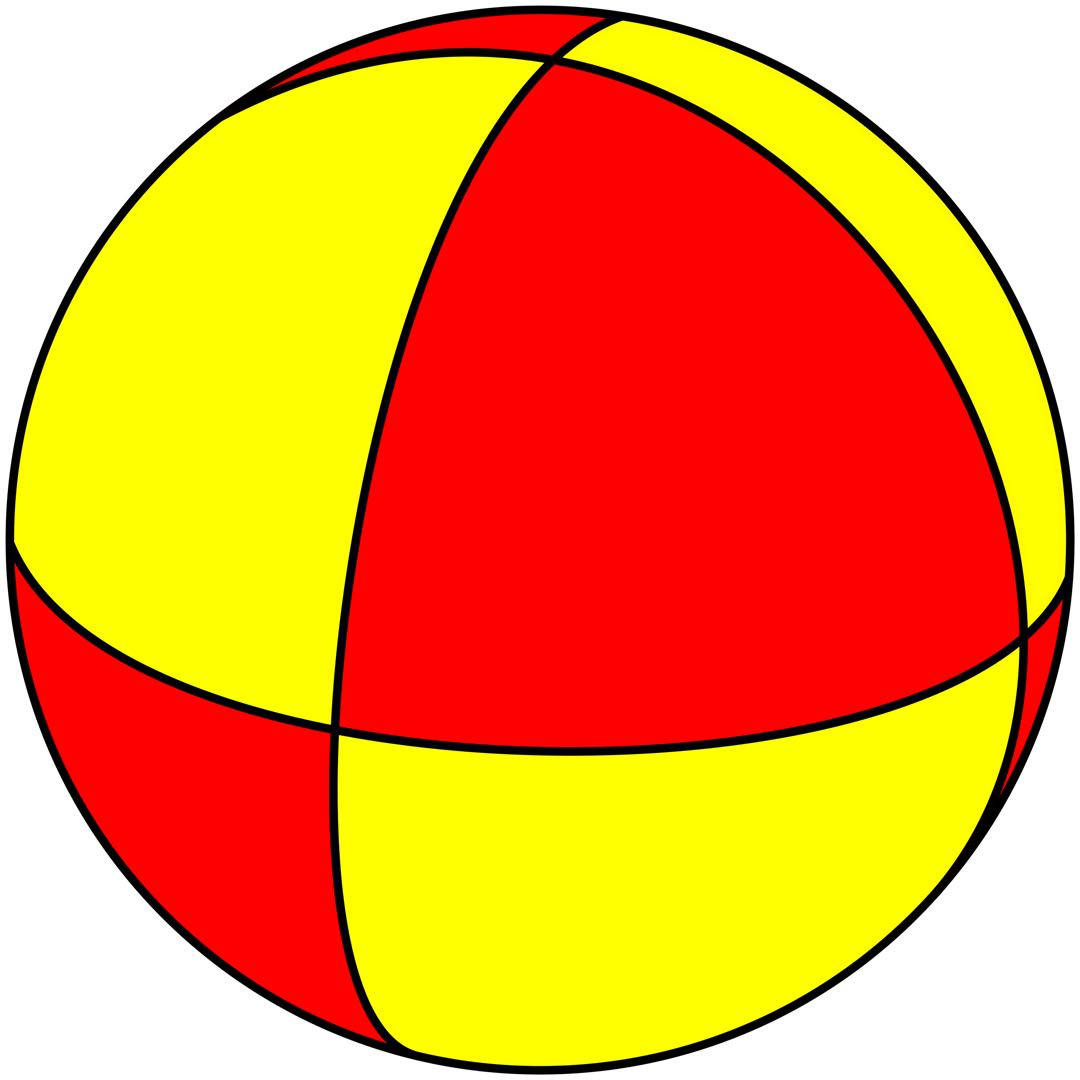
\includegraphics[width=0.9\linewidth]{(2,2,2).jpg}
        \caption{(2,2,2)}
        \label{fig:subim6}
    \end{minipage}
    \begin{minipage}{0.2\linewidth}
        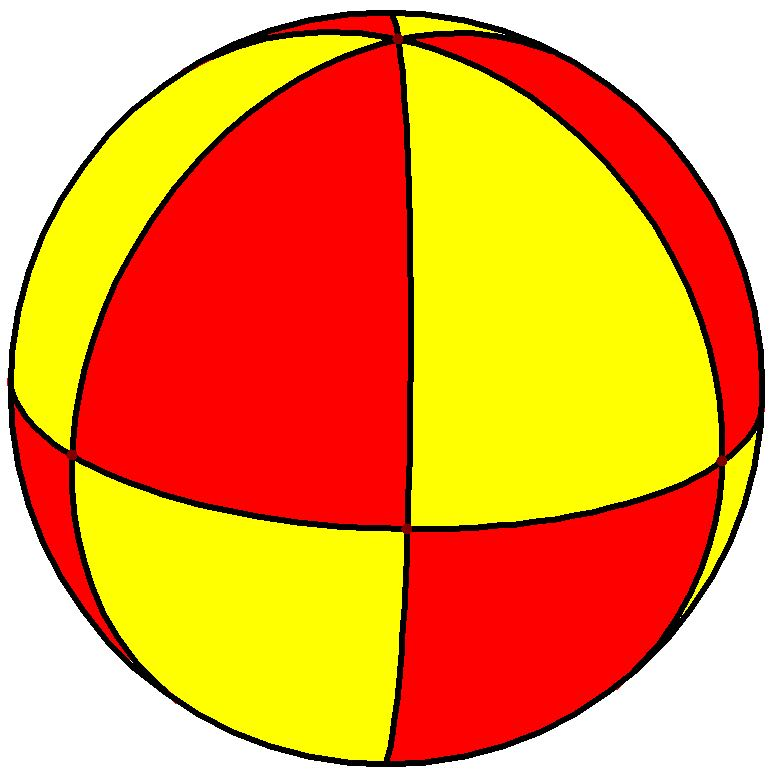
\includegraphics[width=0.9\linewidth]{(2,2,3).jpg}
        \caption{(2,2,3)}
        \label{fig:subim7}
    \end{minipage}
    \begin{minipage}{0.2\linewidth}
        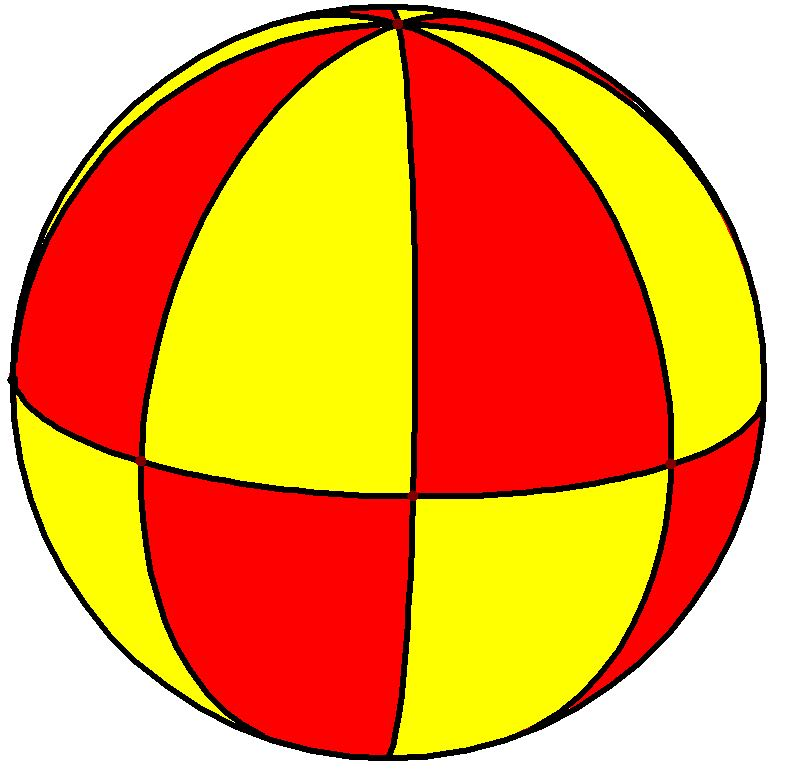
\includegraphics[width=0.9\linewidth]{(2,2,4).jpg}
        \caption{(2,2,4)}
        \label{fig:subim8}
    \end{minipage}
    \caption{The case of (2,2,n)}
    \label{fig:image3}
\end{figure}

\begin{figure}[ht]
    \centering
    \begin{minipage}{0.2\linewidth}
        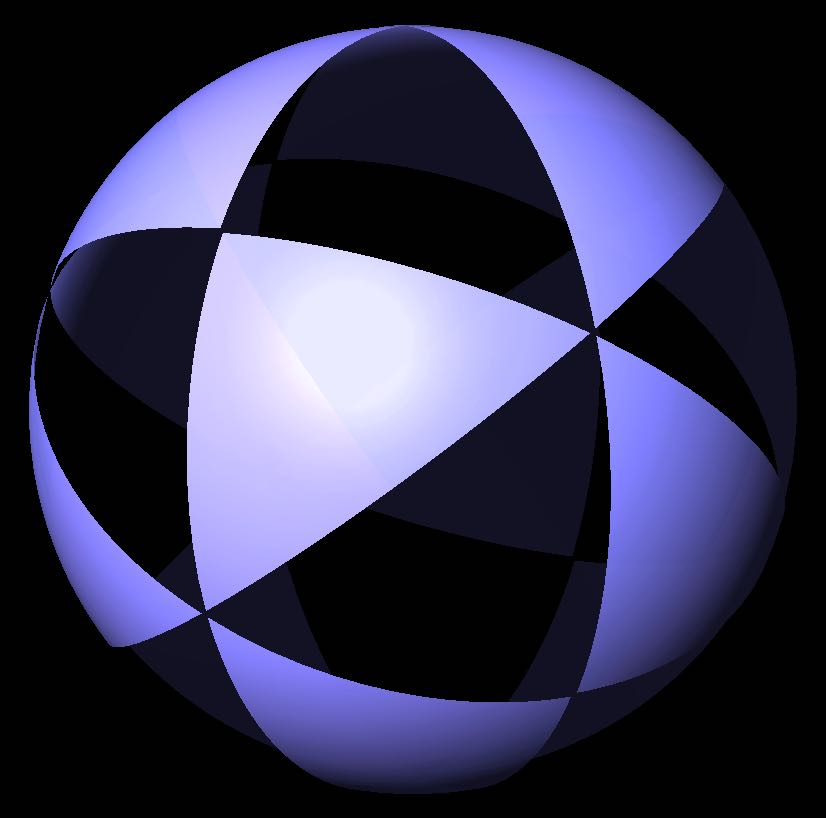
\includegraphics[width=0.9\linewidth]{(2,3,3).jpg}
        \caption{(2,3,3)}
        \label{fig:subim9}
    \end{minipage}
    \begin{minipage}{0.2\linewidth}
        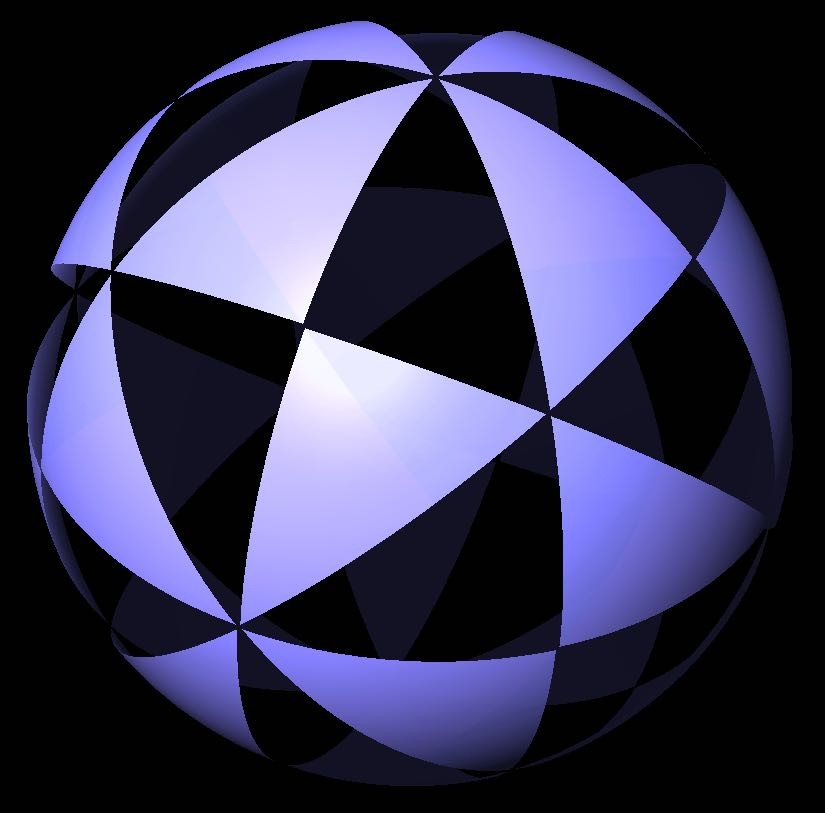
\includegraphics[width=0.9\linewidth]{(2,3,4).jpg}
        \caption{(2,3,4)}
        \label{fig:subim10}
    \end{minipage}
    \begin{minipage}{0.2\linewidth}
        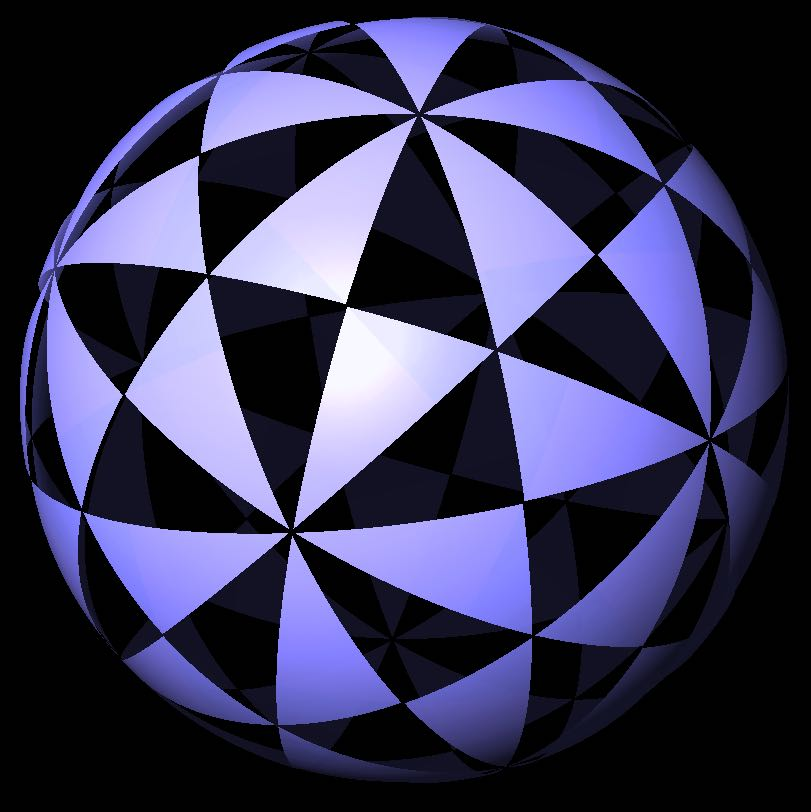
\includegraphics[width=0.9\linewidth]{(2,3,5).jpg}
        \caption{(2,3,5)}
        \label{fig:subim11}
    \end{minipage}
    \caption{The other case}
    \label{fig:image12}
\end{figure}
%=================================LZP===================
\subsection{Hyperbolic Space}
Similiar to the equation before, we have:
\[\frac{1}{p} + \frac{1}{q} + \frac{1}{r} < 1\]
As p,q,r are positive integers $\geq$ 2.

Notice that we have endless options for $p$,$q$,$r$ if they are big enough. But do all these possible hyperbolic triangles indeed exist in the hyperbolic model? The answer is YES! We can just fix two angles of the triangle, and try to change the third angle and see whether it will vary continuously. The idea is summarized in the following theorem and see Figure: \ref{Example} as animation.

\begin{Thm}
    for any $\alpha$,$\beta$,$\gamma$, satisfied $\alpha+\beta+\gamma<\pi$,
    We can find such a hyperbolic triangle in hyperbolic model.
\end{Thm}
\begin{proof}
    Here we will show the sketch of the proof in Poincare's disc model:

    We find such triangles by progressively determining the angle.
    first fixed a point in the origin, call it $A$, and let $t \vcentcolon AB$(notice that We define length AB in Euclidean length)
    Draw the ray with angle $\alpha$ to AB.(Figure: \ref{step1})
    Next, draw the ray with angle $\beta-\frac{\pi}{2}$ to the right positive semi-axis. We get $\beta$.(Figure: \ref{step2})

    Then we call the last angle of $ABC$ $\gamma(t)$, it will changed with t.

    When $t\rightarrow 0,\gamma(t)\rightarrow \pi-\alpha-\beta$, it is the maximum angle $\gamma(t)$ can reach.

    When $t\rightarrow \infty,\gamma(t)\rightarrow 0$, it is the minimum angle $\gamma(t)$ can reach.

    Following the continuity of $\gamma(t)$ with respect to the variation of $t$, by Intermedian Theorem,
    we obtain that any angle required by $\gamma(t)$ can be obtained by transforming $t$.(Figure: \ref{gamma})
\end{proof}
\newpage
\begin{figure}[ht]%给一些图片的例子
    \centering
    \begin{minipage}{0.25\linewidth}
        \centering
        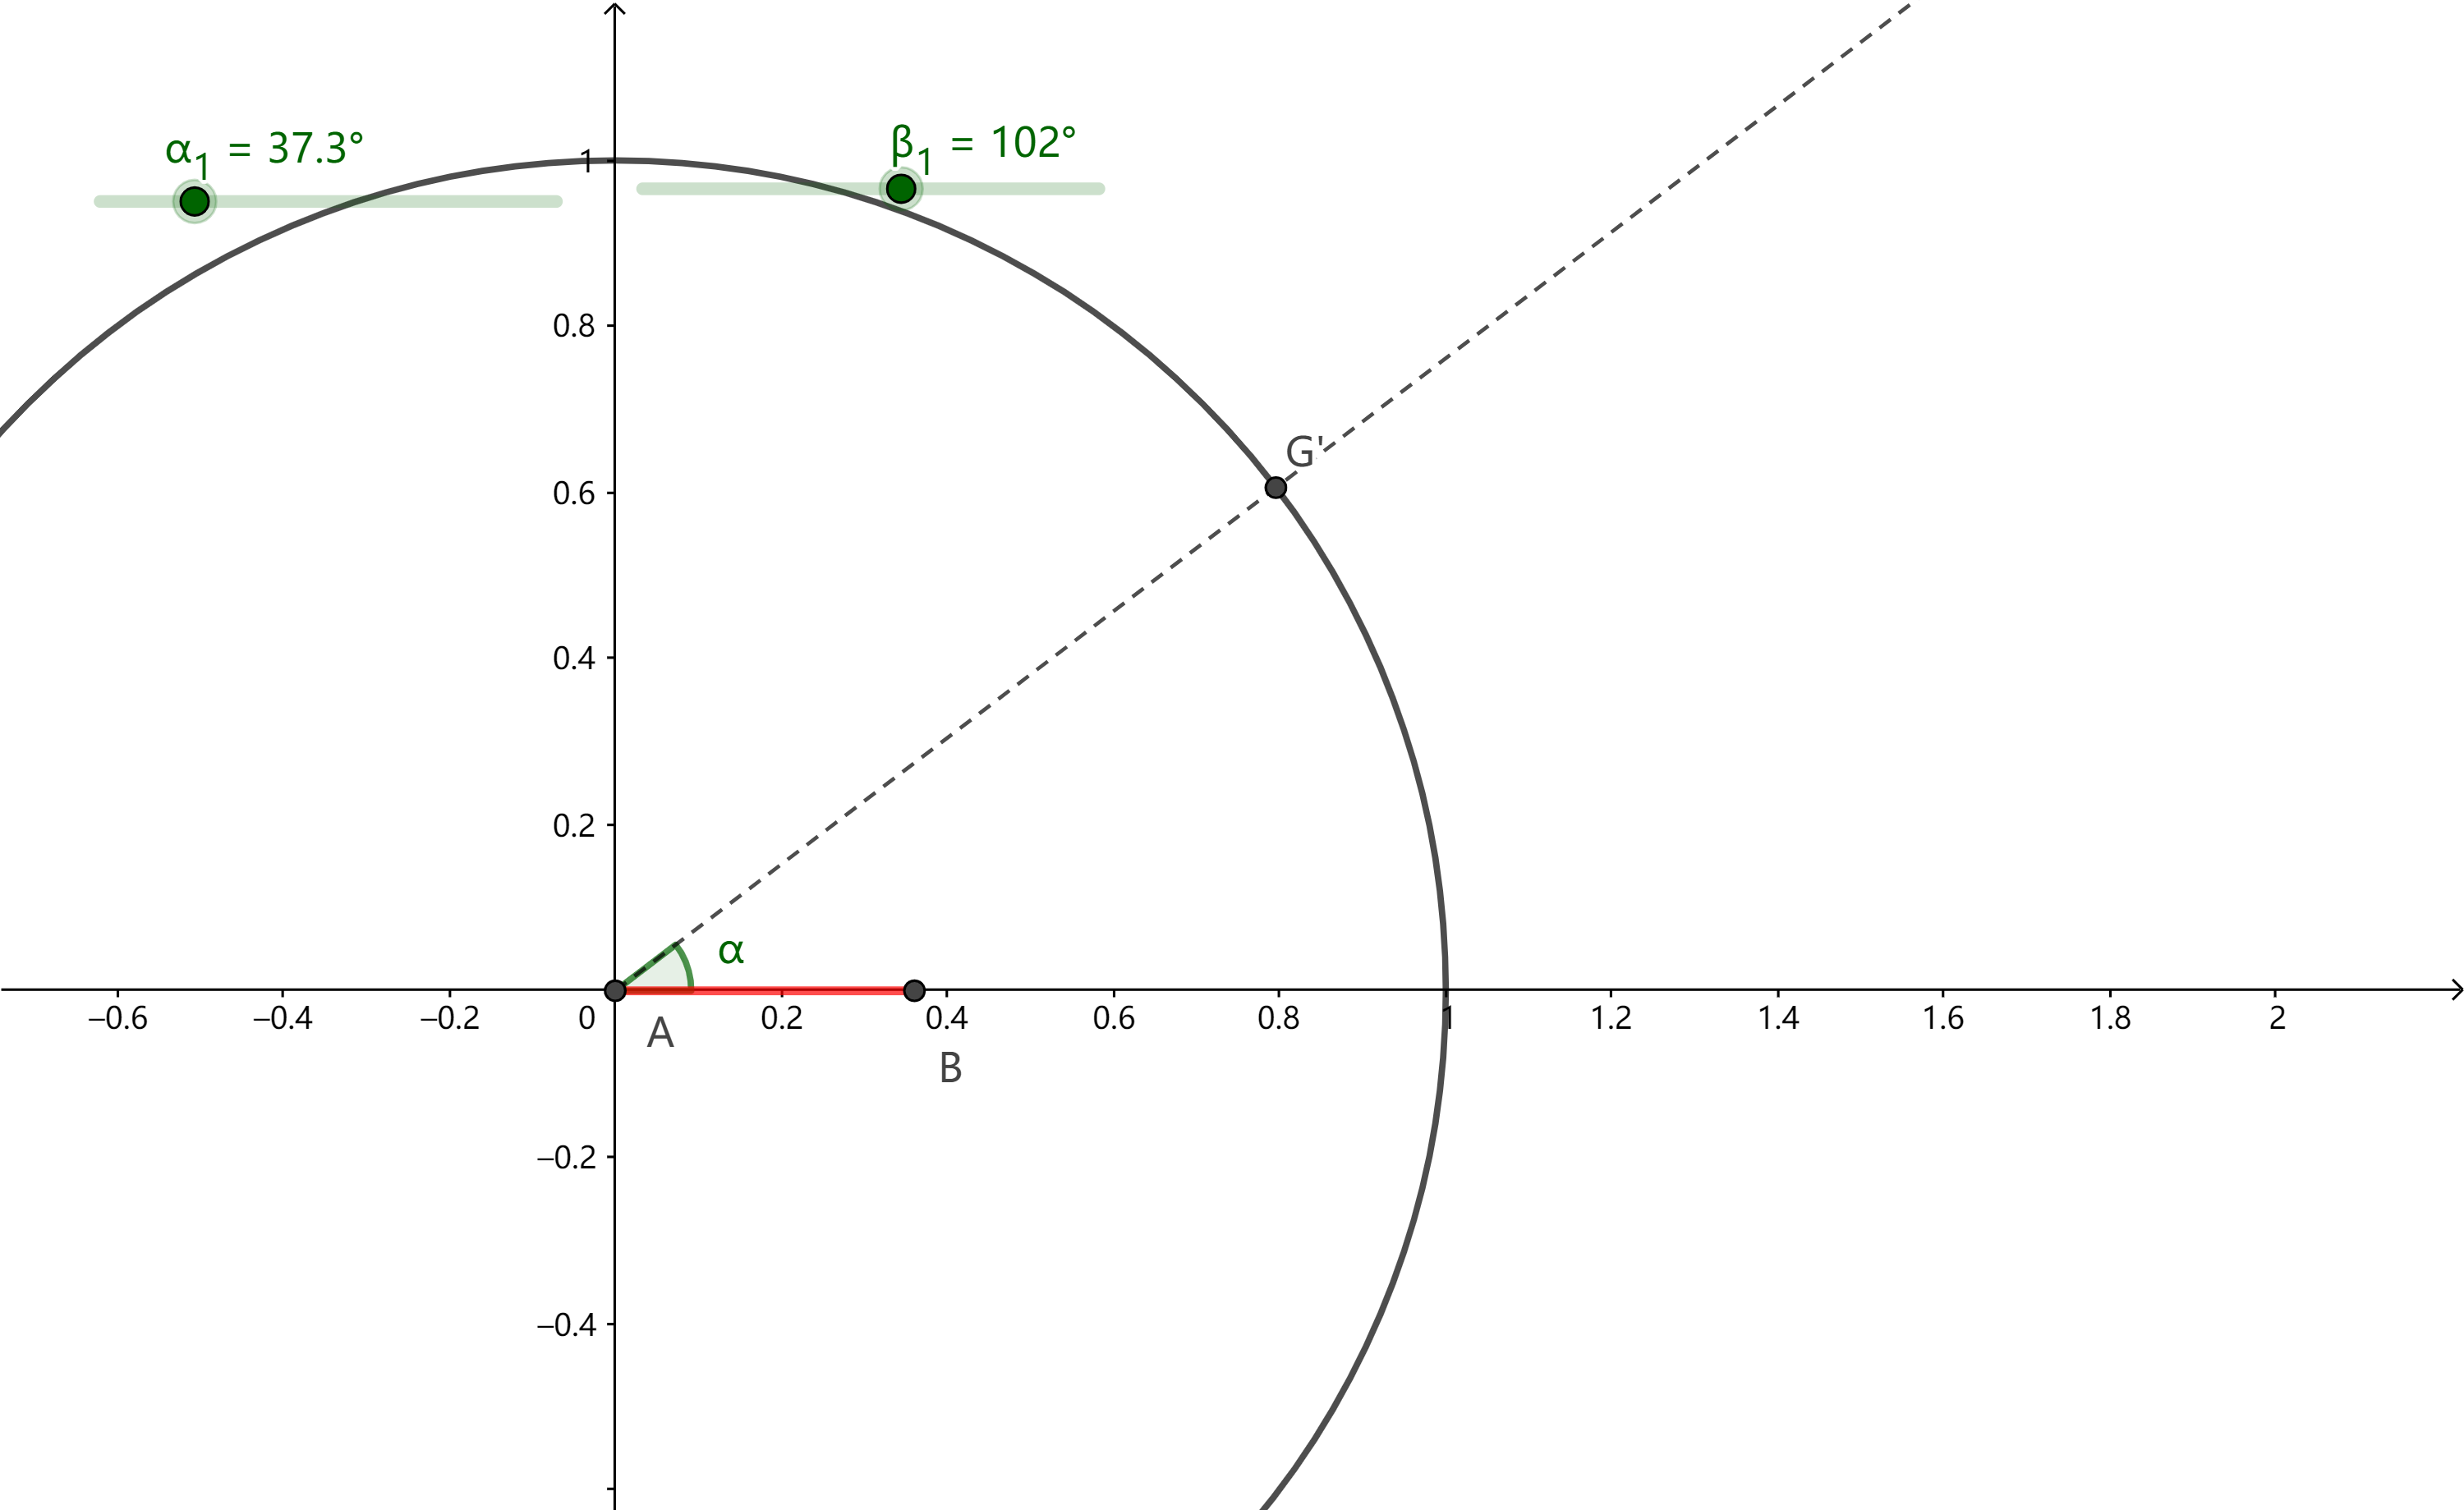
\includegraphics[width={0.9\linewidth}]{B9.png}
        \caption{}
        \label{step1}
    \end{minipage}
    \begin{minipage}{0.25\linewidth}
        \centering
        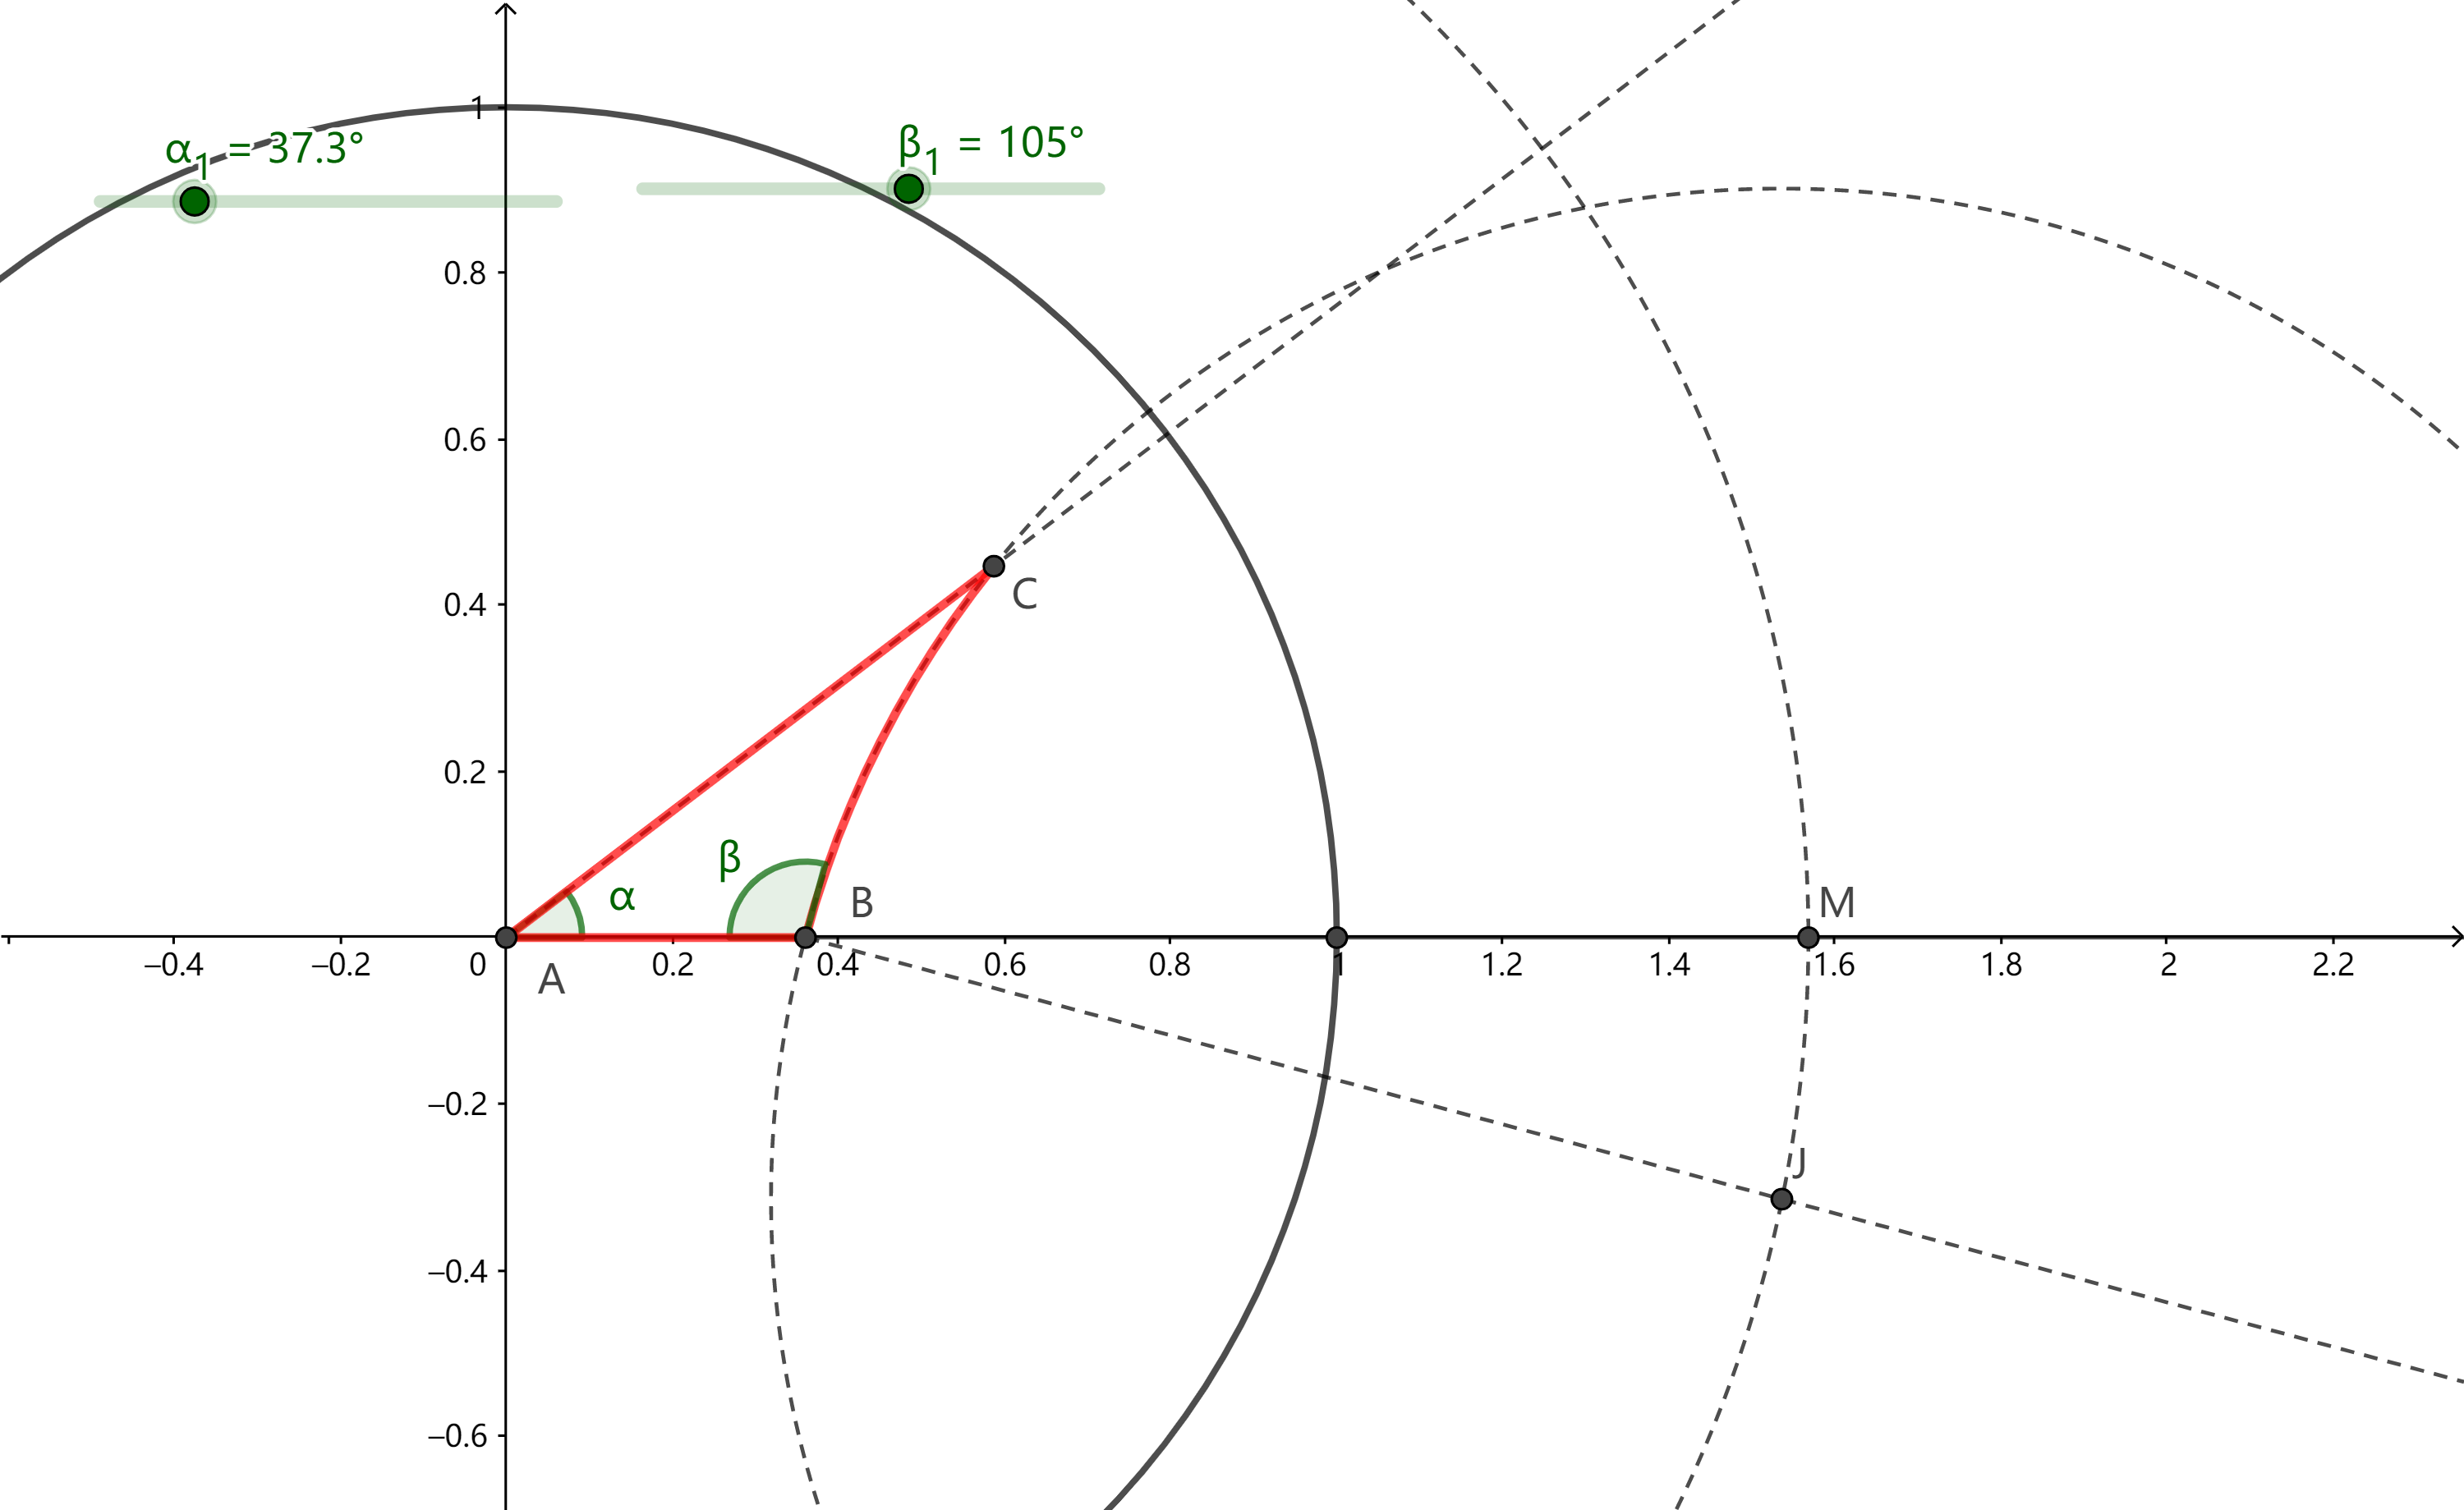
\includegraphics[width={0.9\linewidth}]{B7.png}
        \caption{}
        \label{step2}
    \end{minipage}
\end{figure}

\begin{figure}[htbp]%给一些图片的例子
    \centering
    \begin{minipage}{0.25\linewidth}
        \centering
        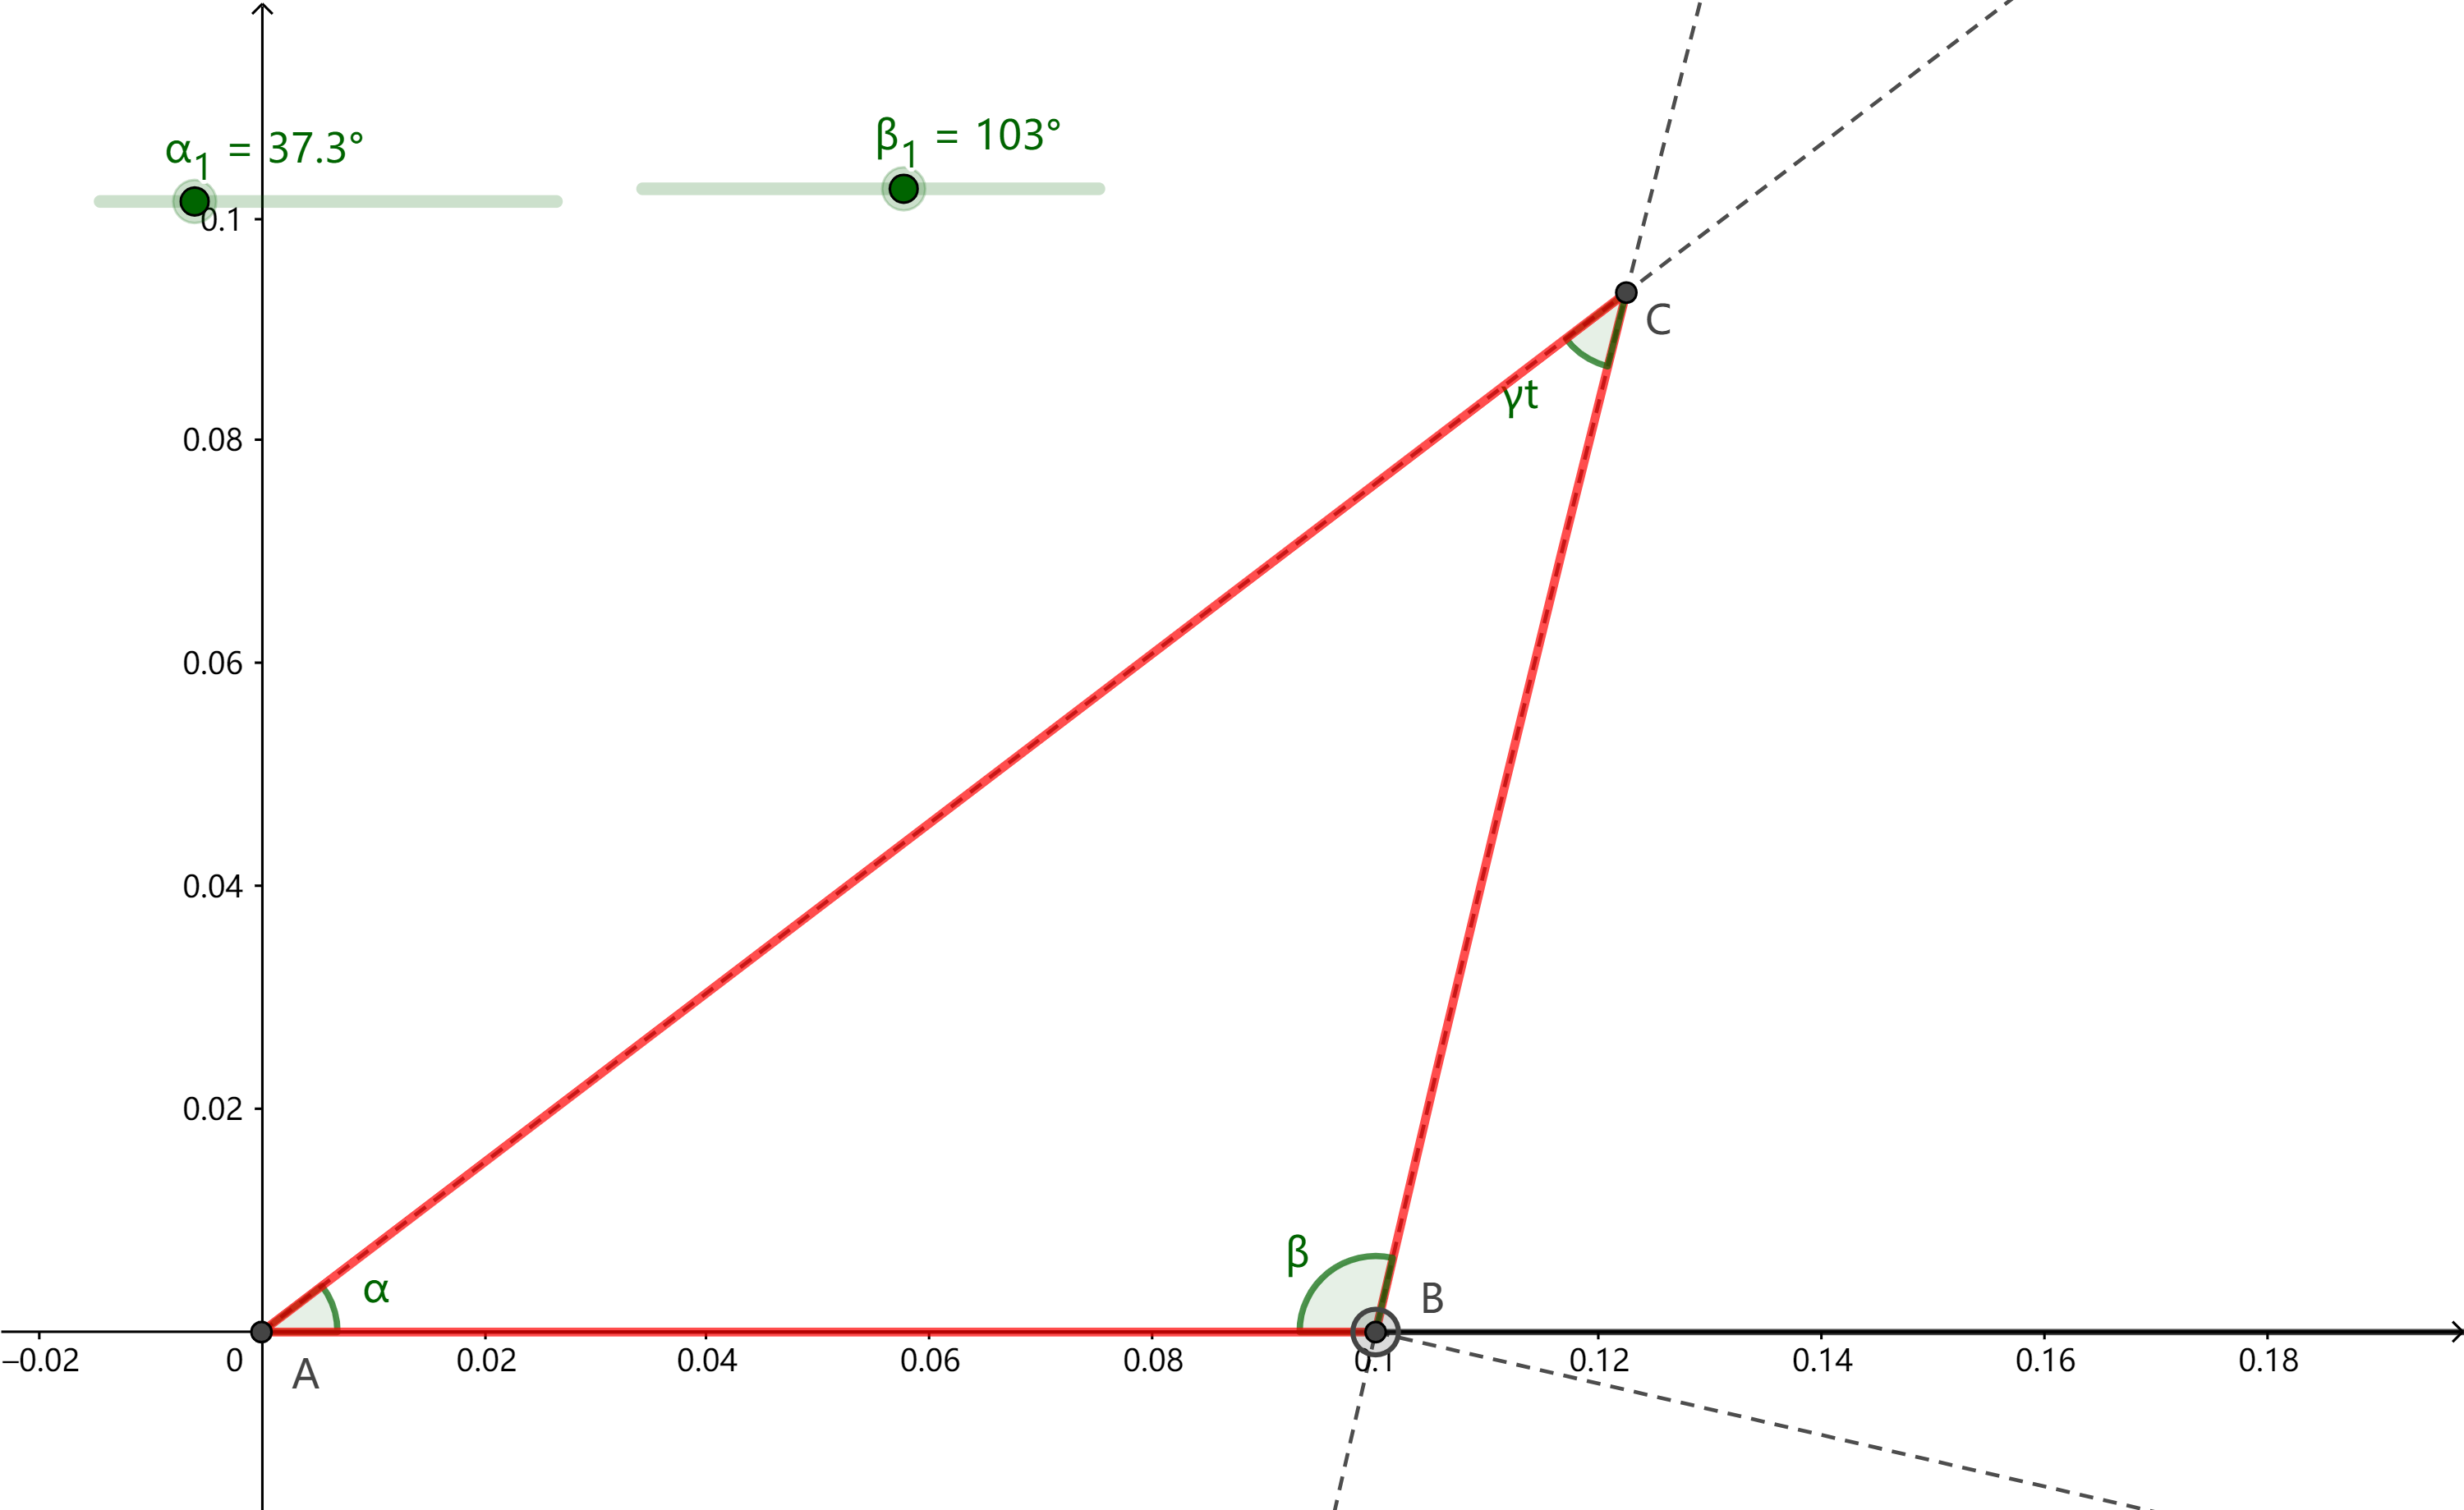
\includegraphics[width={0.9\linewidth}]{B6.png}
        \caption*{$t=0.1$}
    \end{minipage}
    \begin{minipage}{0.25\linewidth}
        \centering
        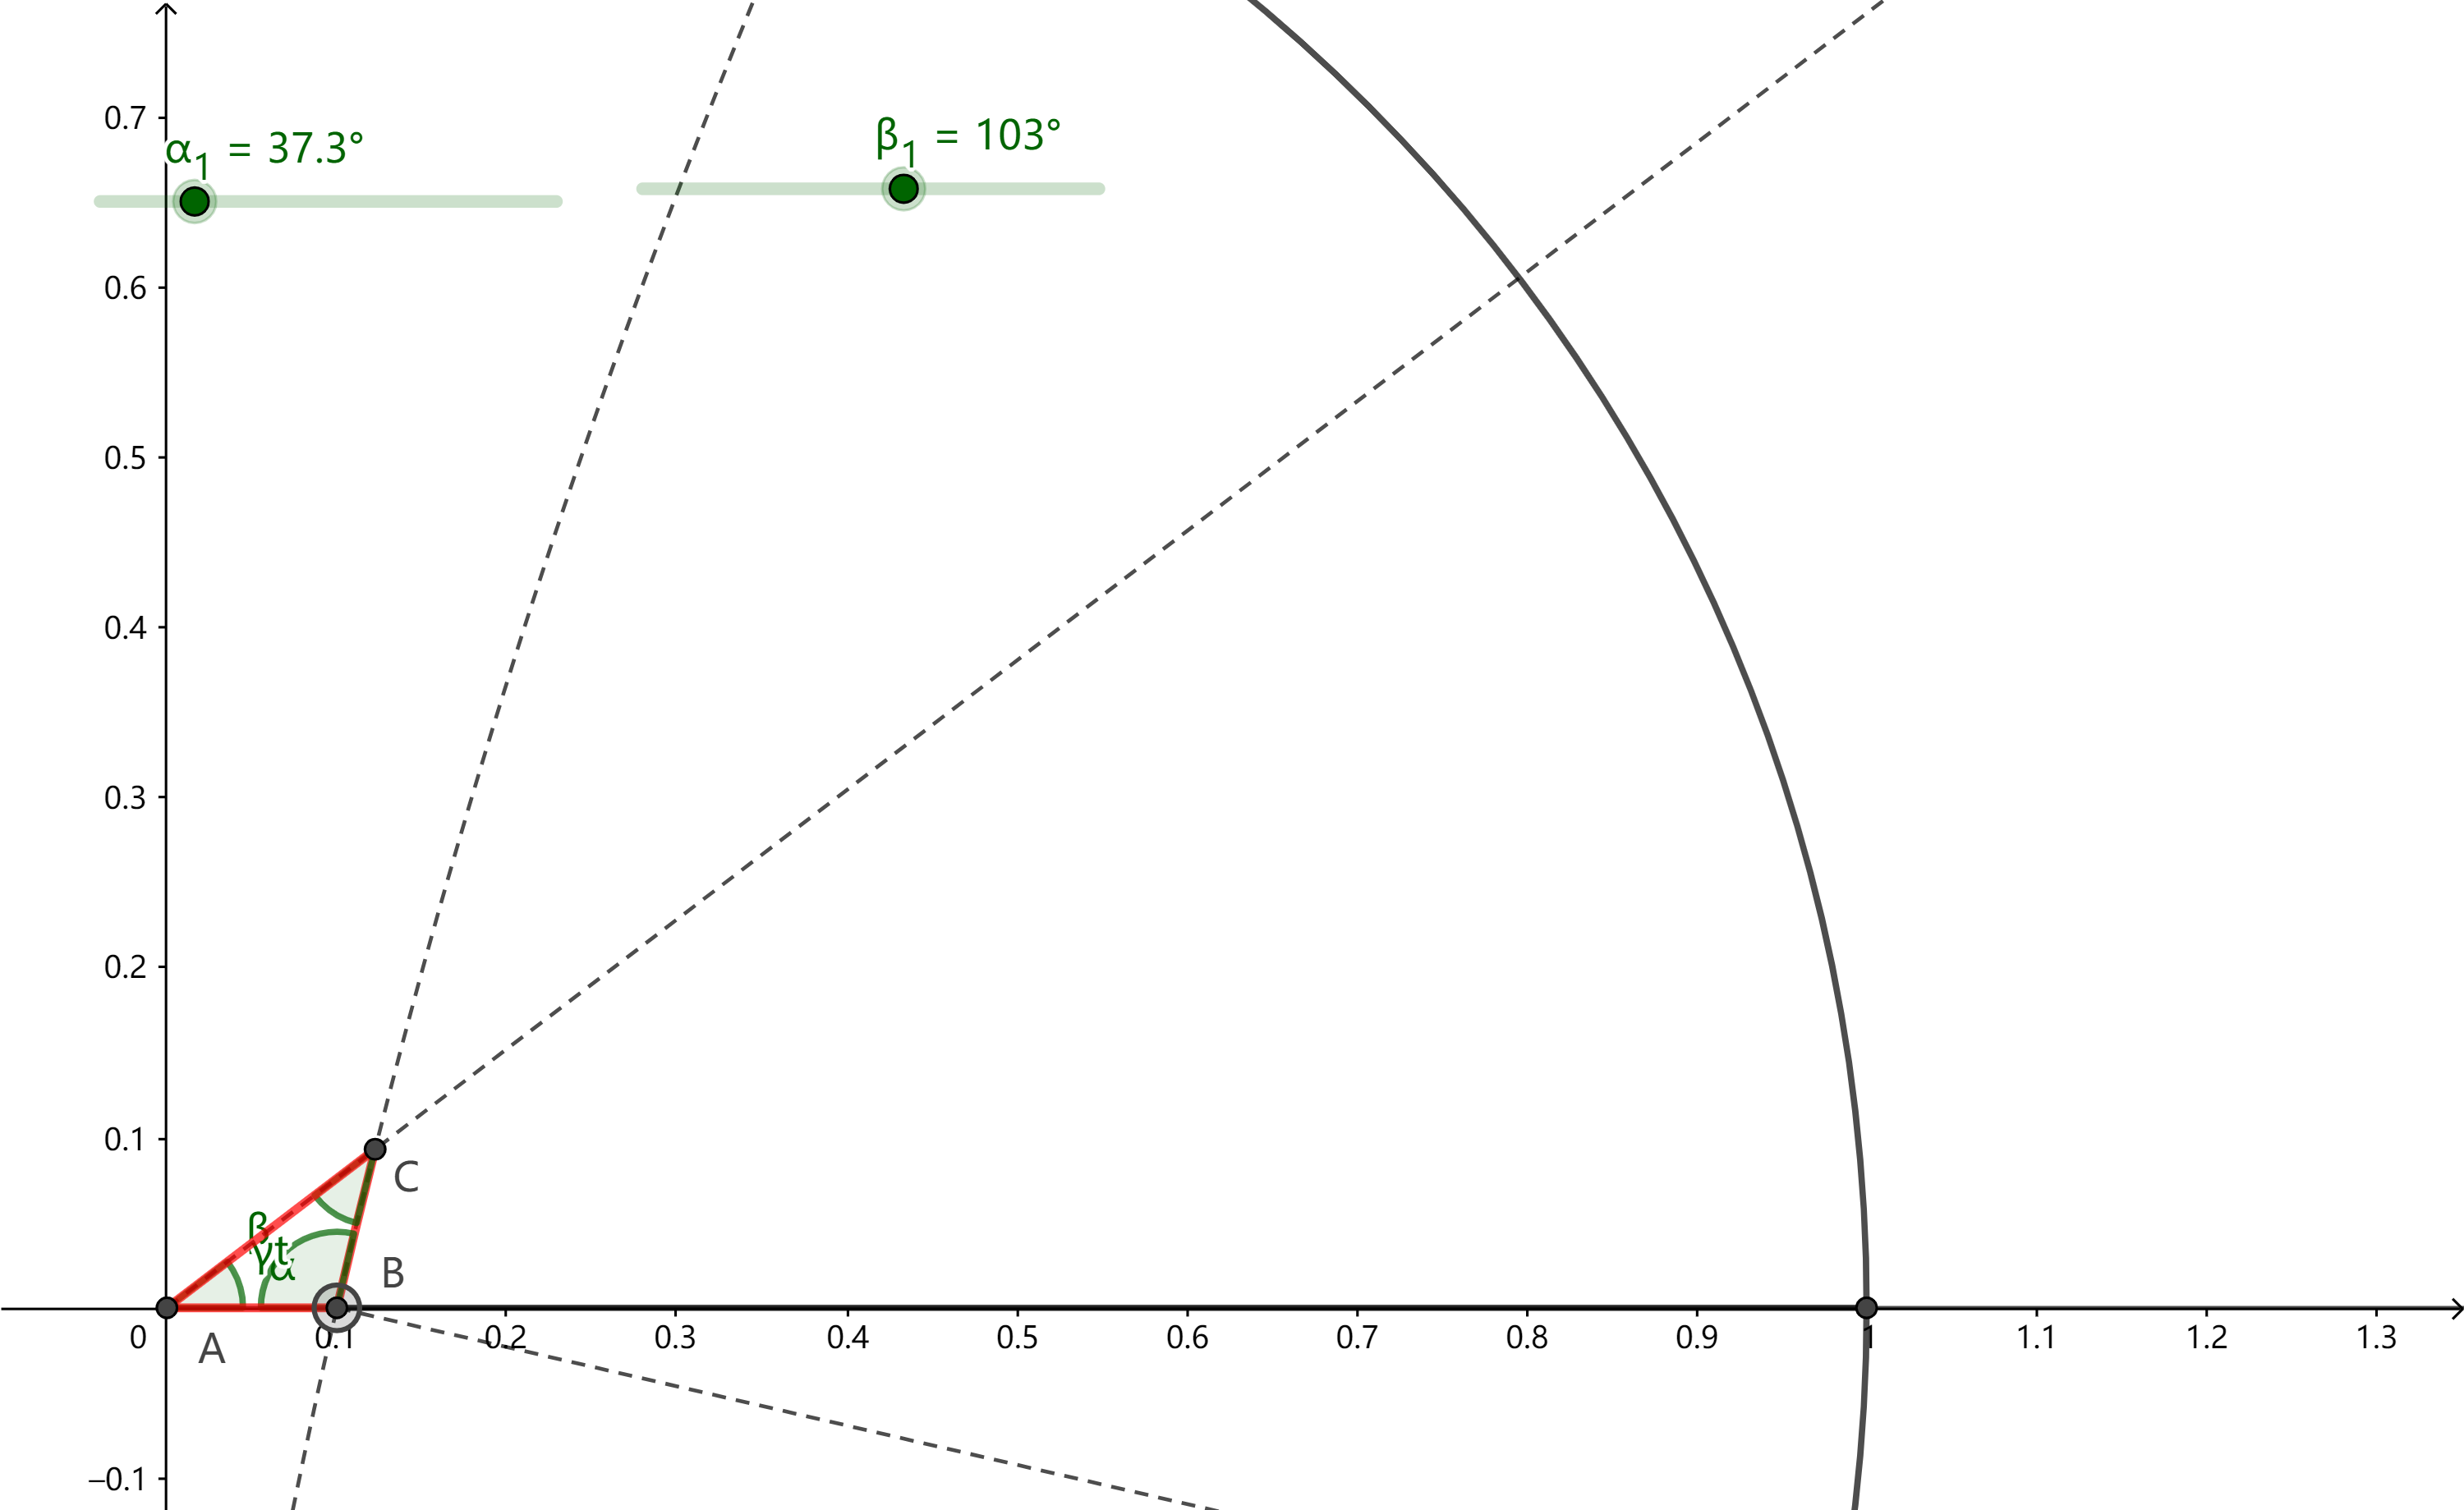
\includegraphics[width={0.9\linewidth}]{B5.png}
        \caption*{$t=0.1$}
    \end{minipage}
    \begin{minipage}{0.25\linewidth}
        \centering
        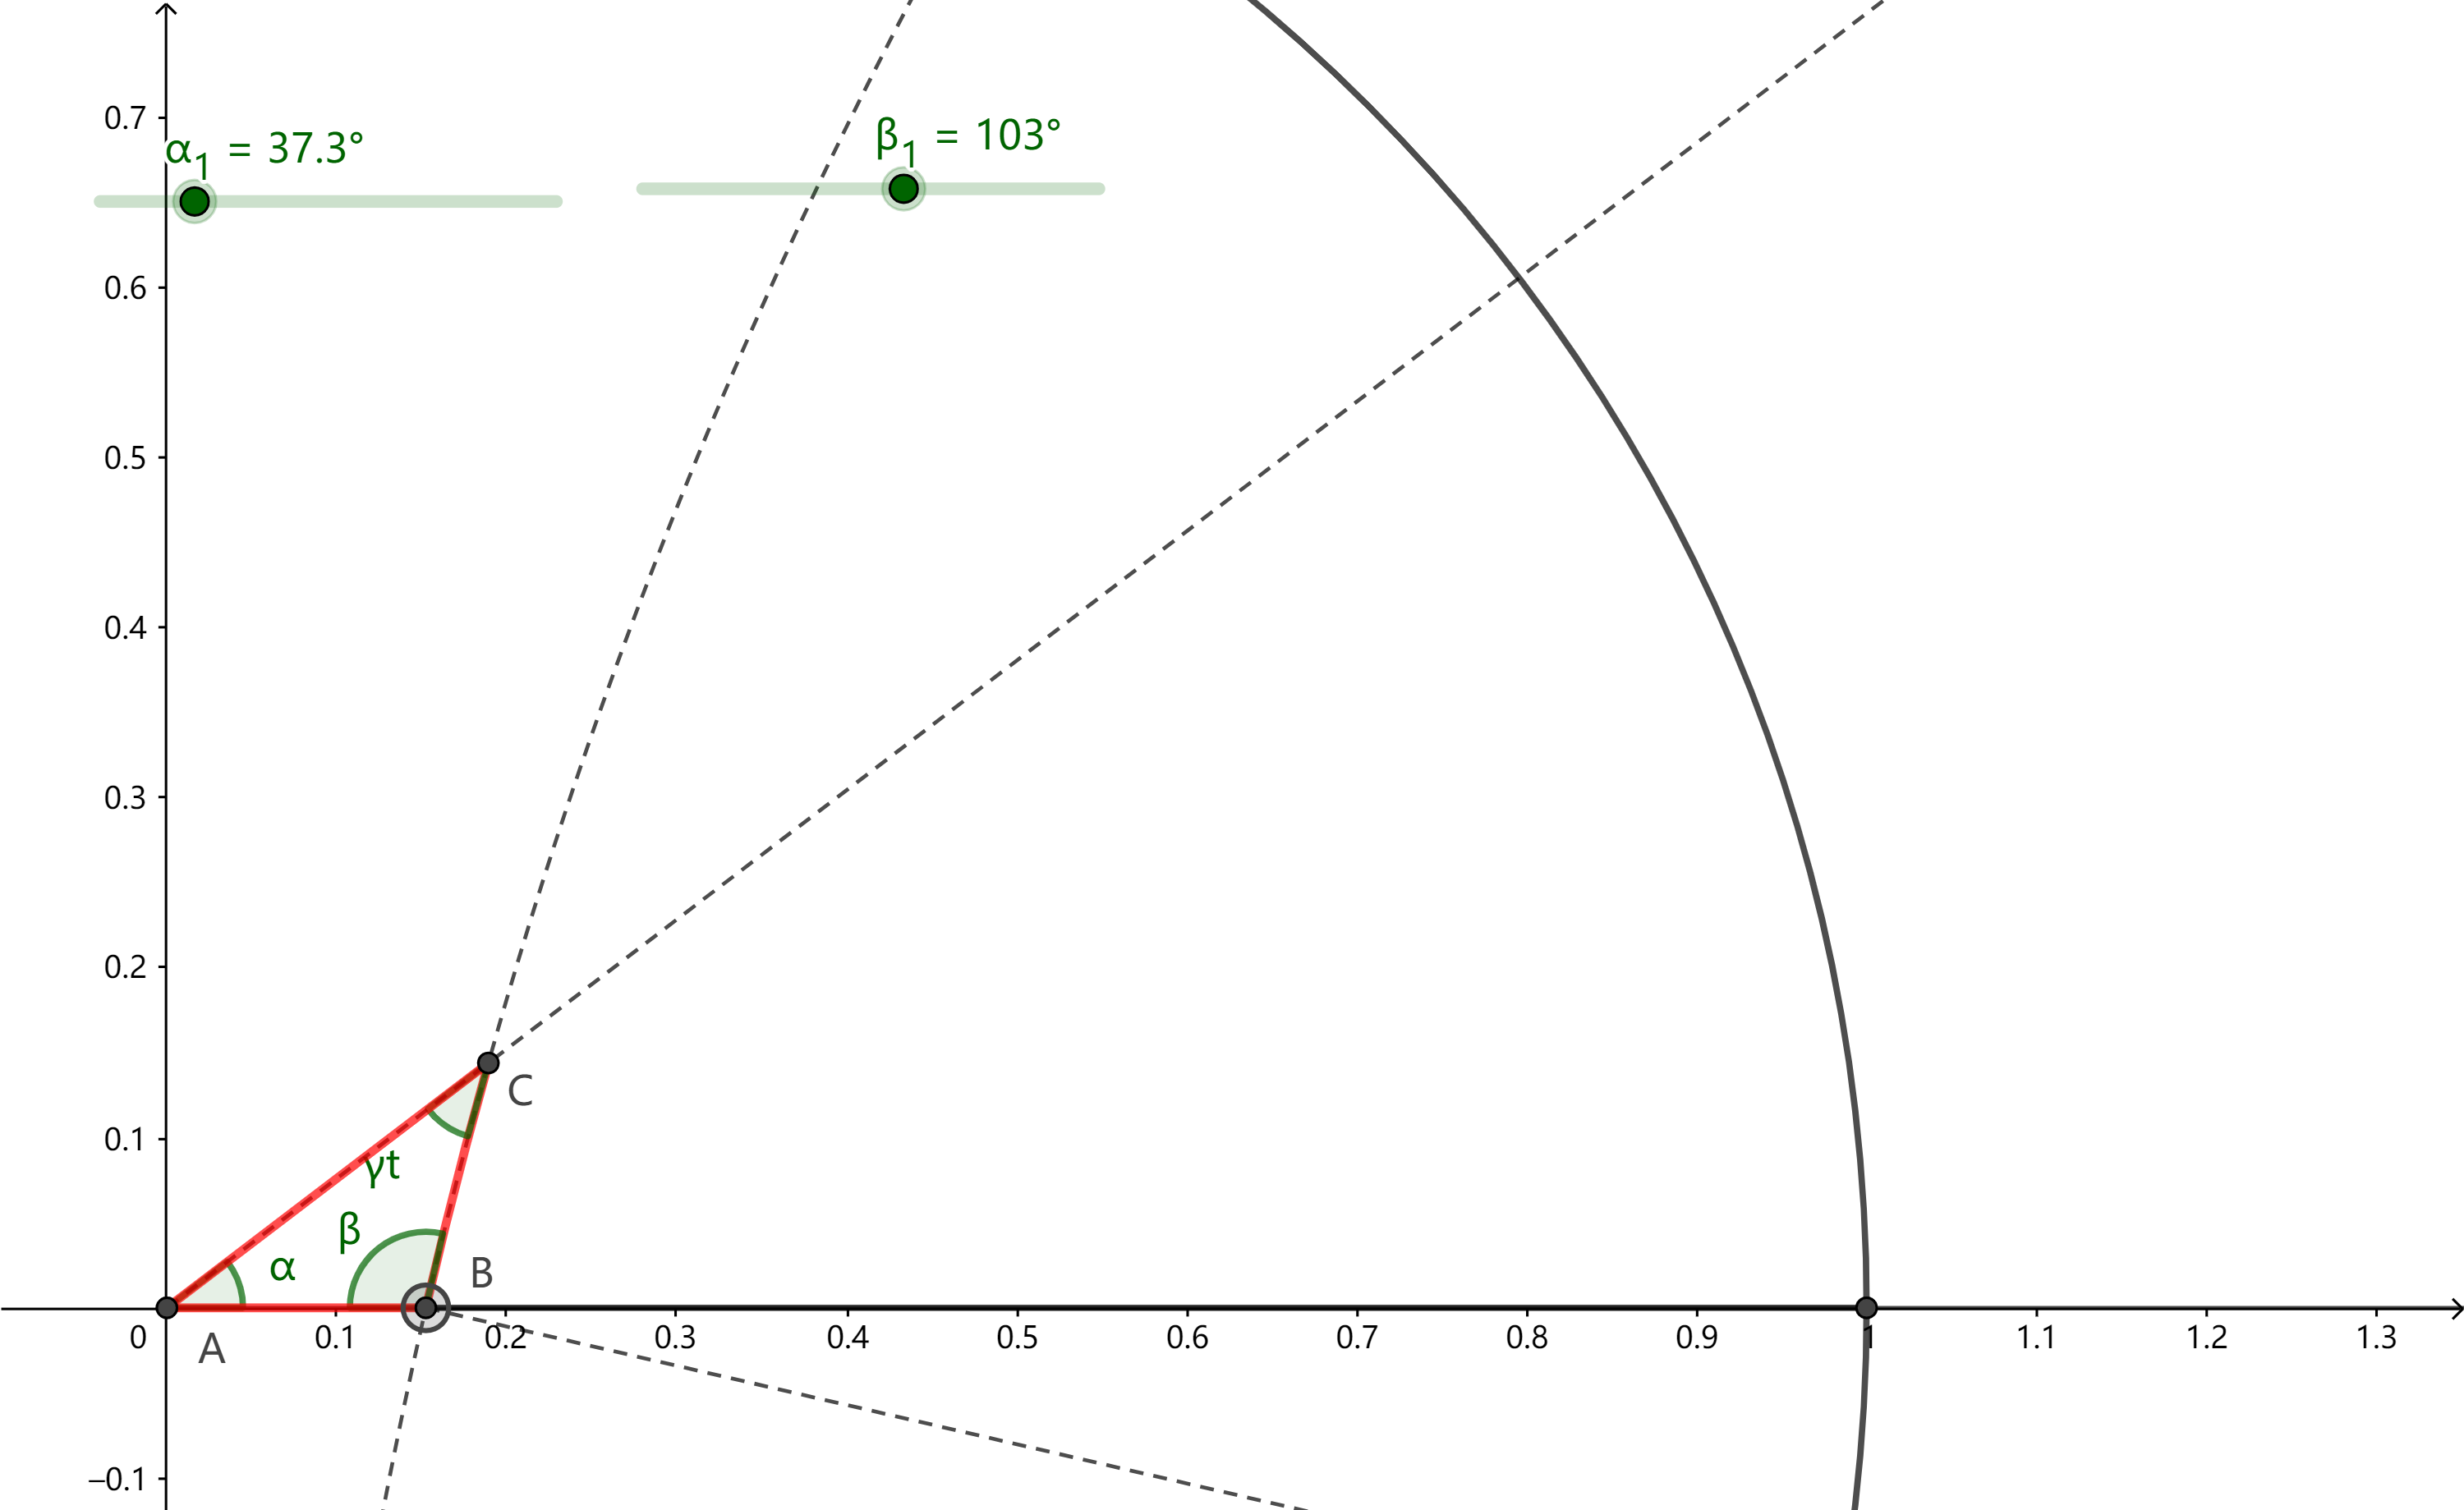
\includegraphics[width={0.9\linewidth}]{B4.png}
        \caption*{$t=0.15$}
    \end{minipage}
    \begin{minipage}{0.25\linewidth}
        \centering
        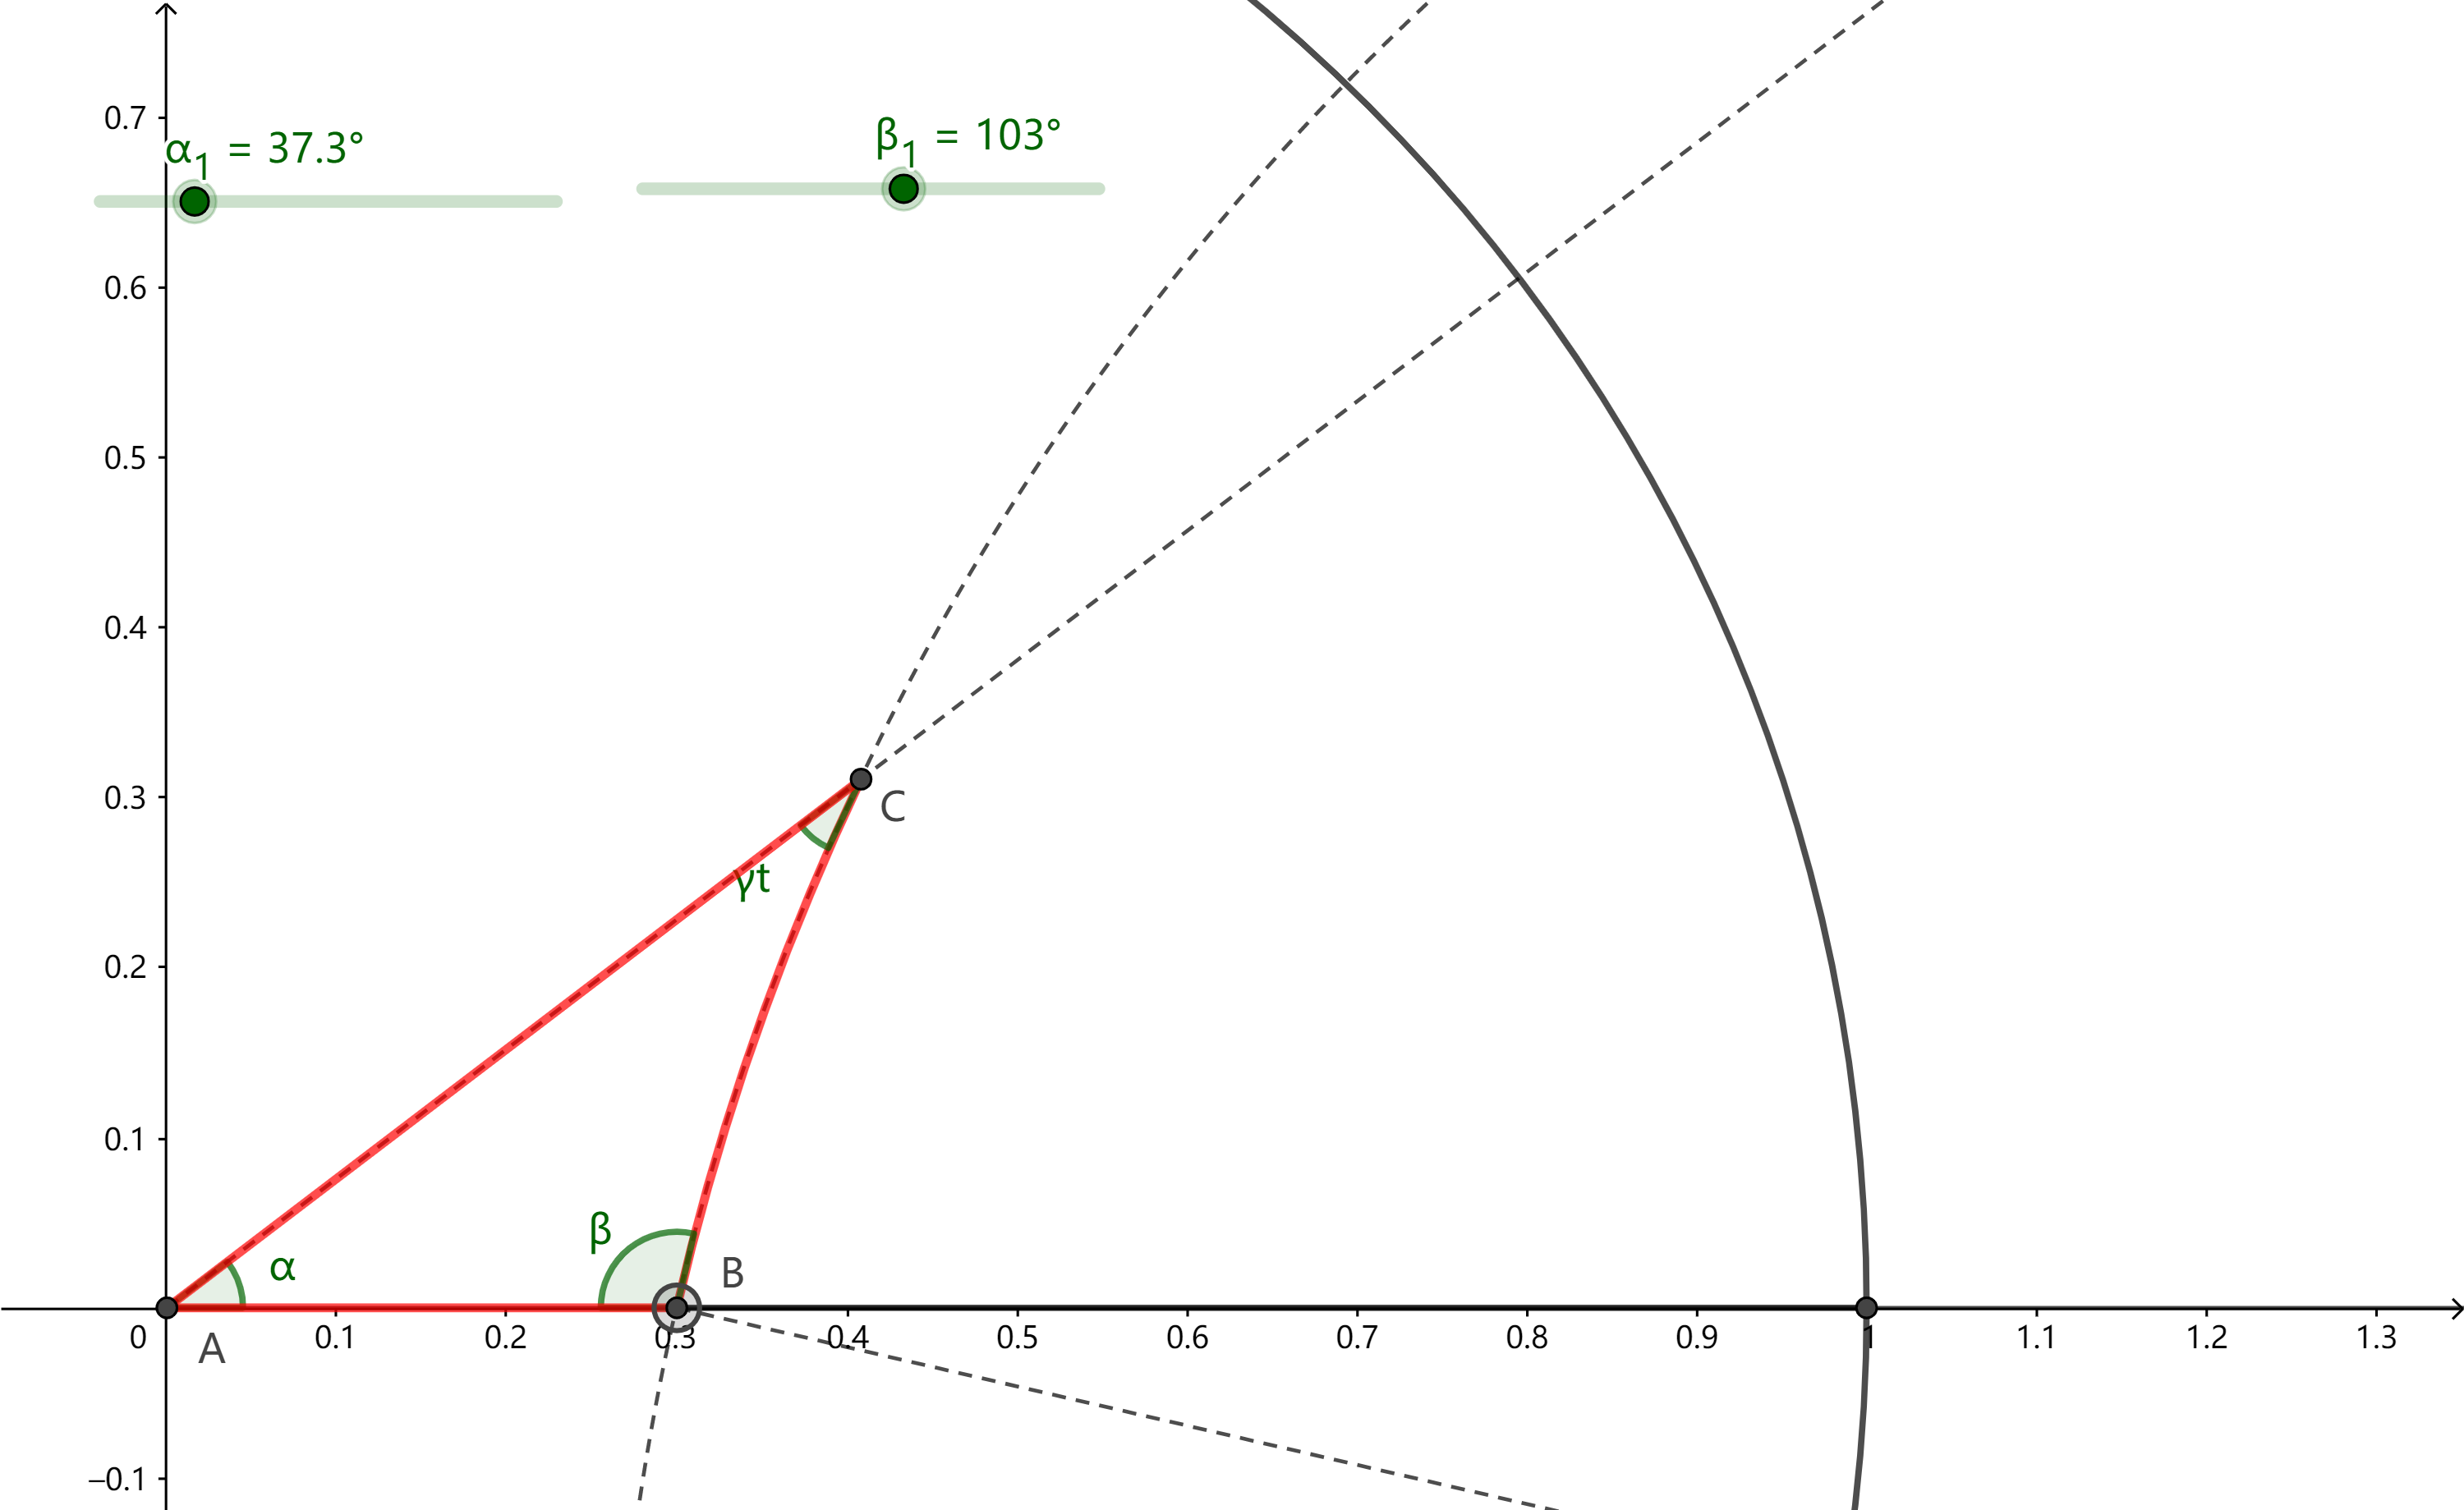
\includegraphics[width={0.9\linewidth}]{B3.png}
        \caption*{$t=0.3$}
    \end{minipage}
    \begin{minipage}{0.25\linewidth}
        \centering
        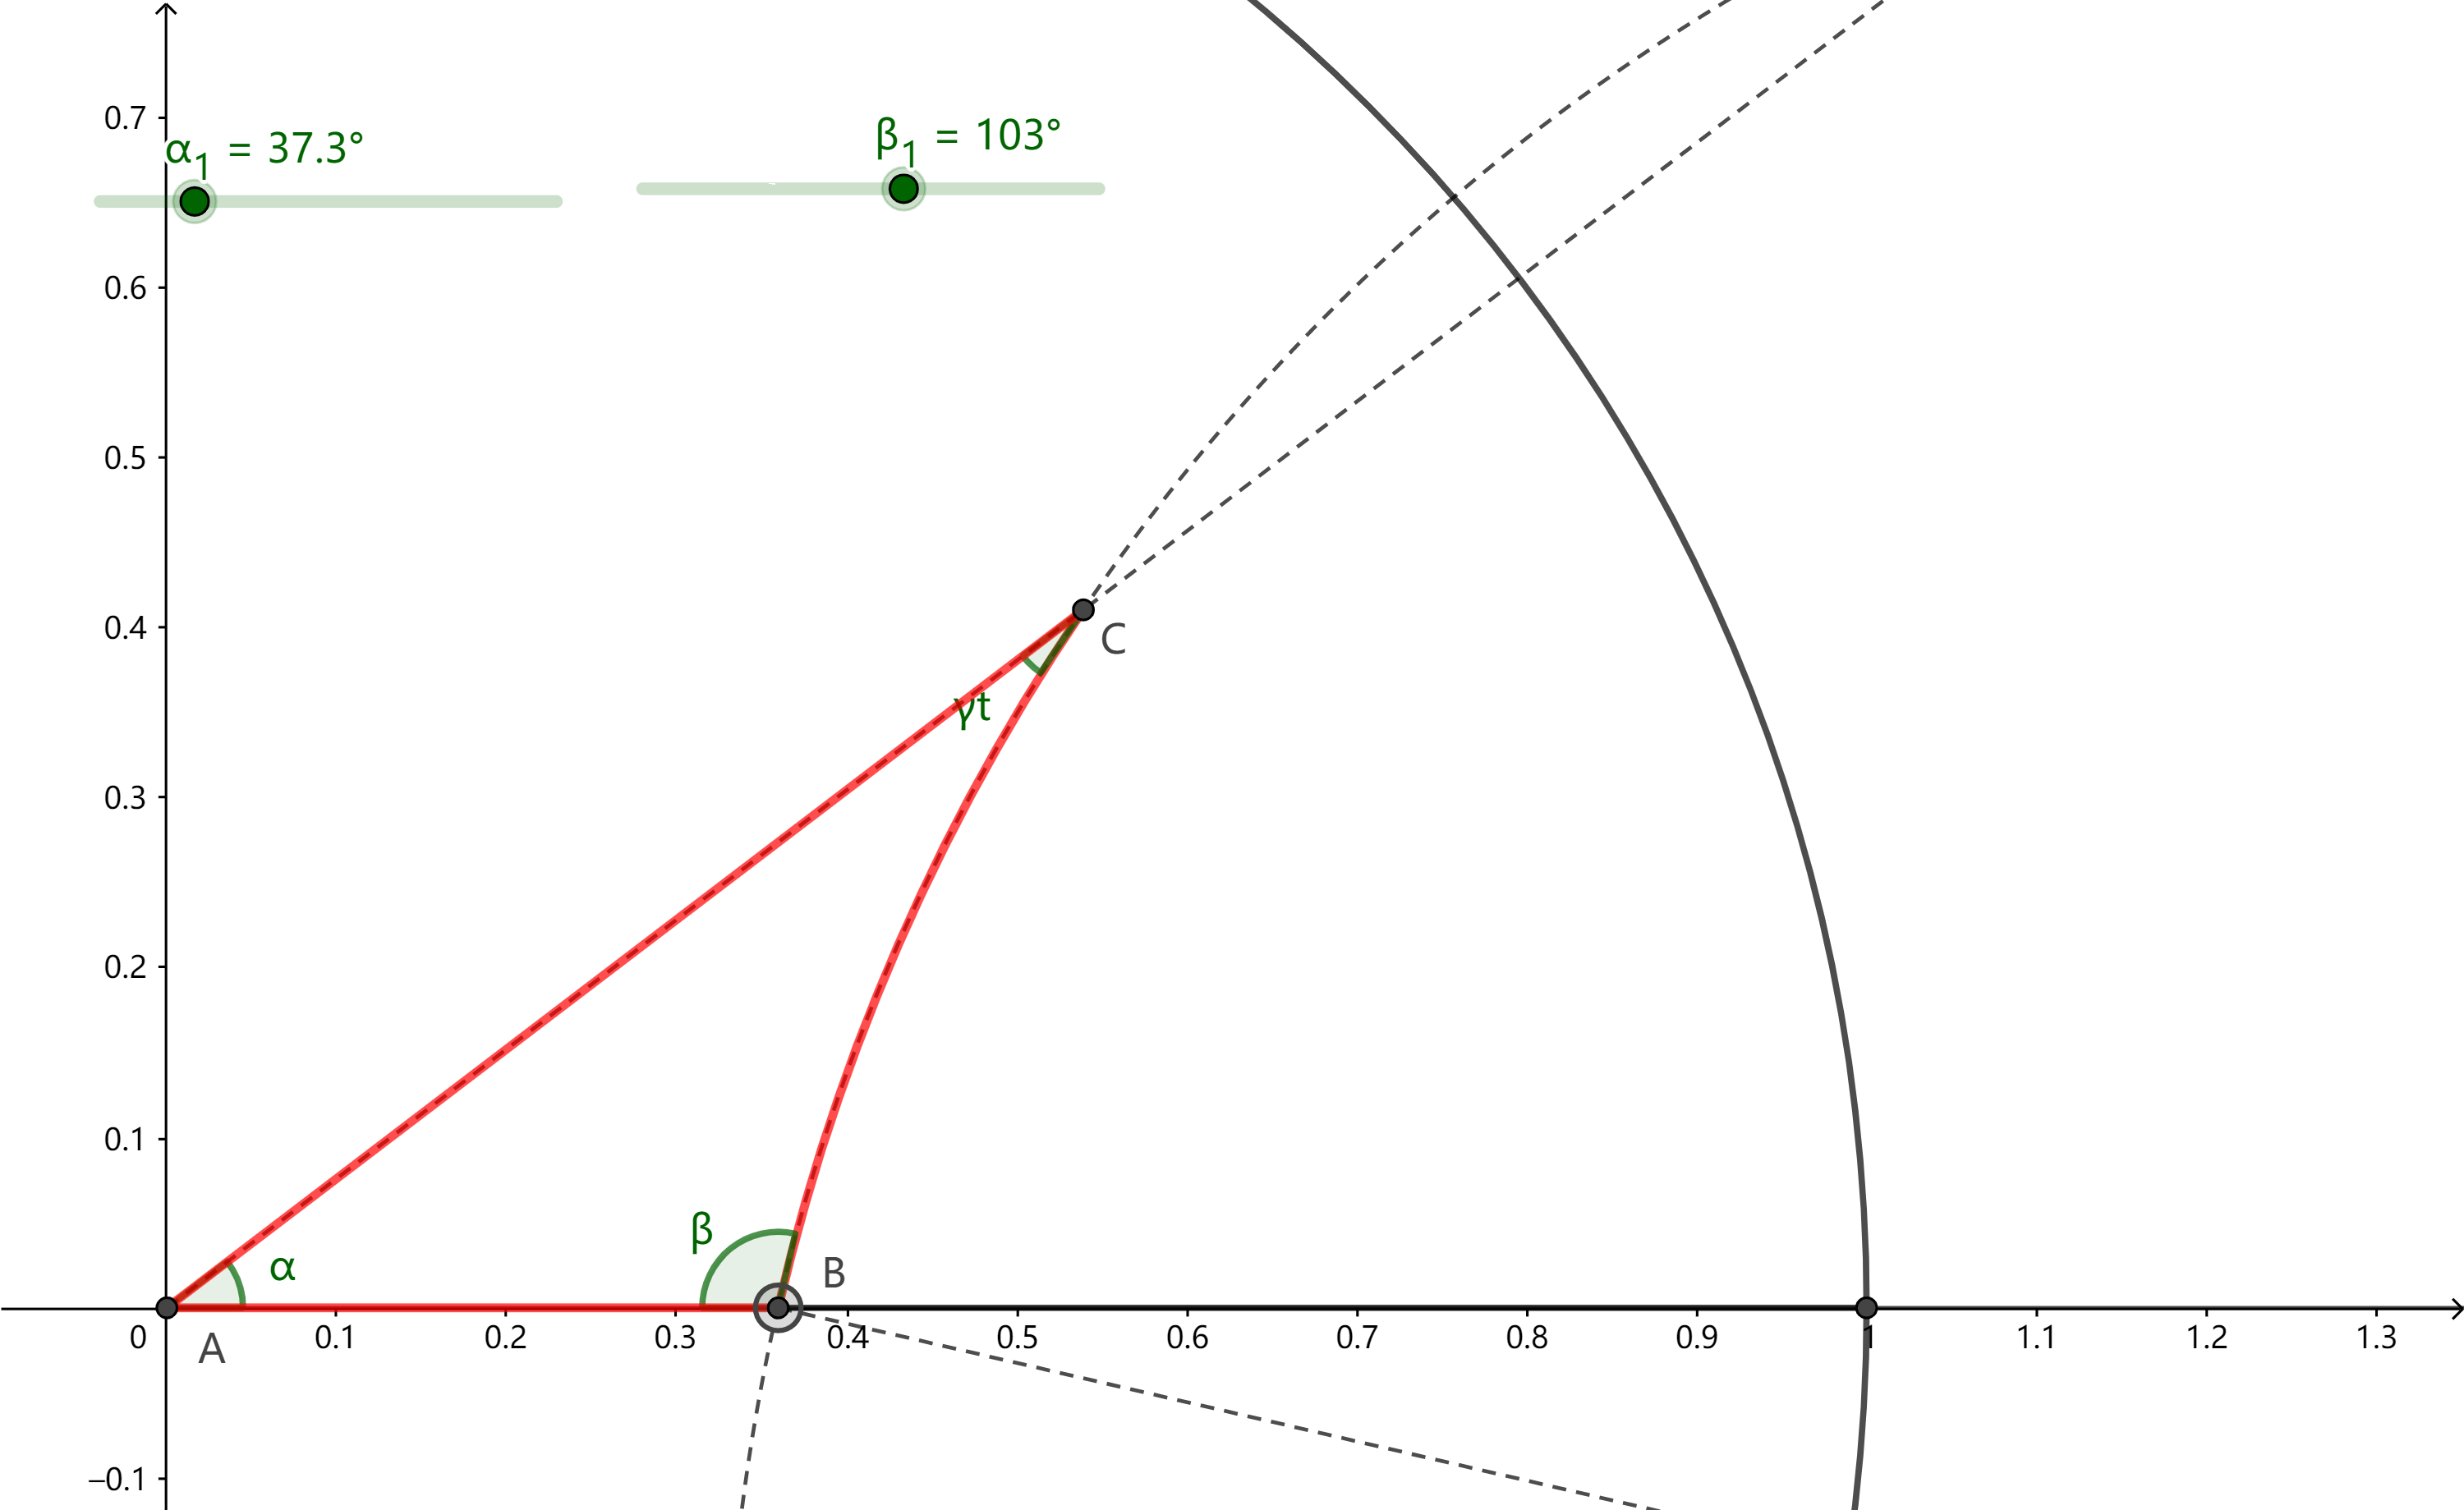
\includegraphics[width={0.9\linewidth}]{B2.png}
        \caption*{$t=0.37$}
    \end{minipage}
    \begin{minipage}{0.25\linewidth}
        \centering
        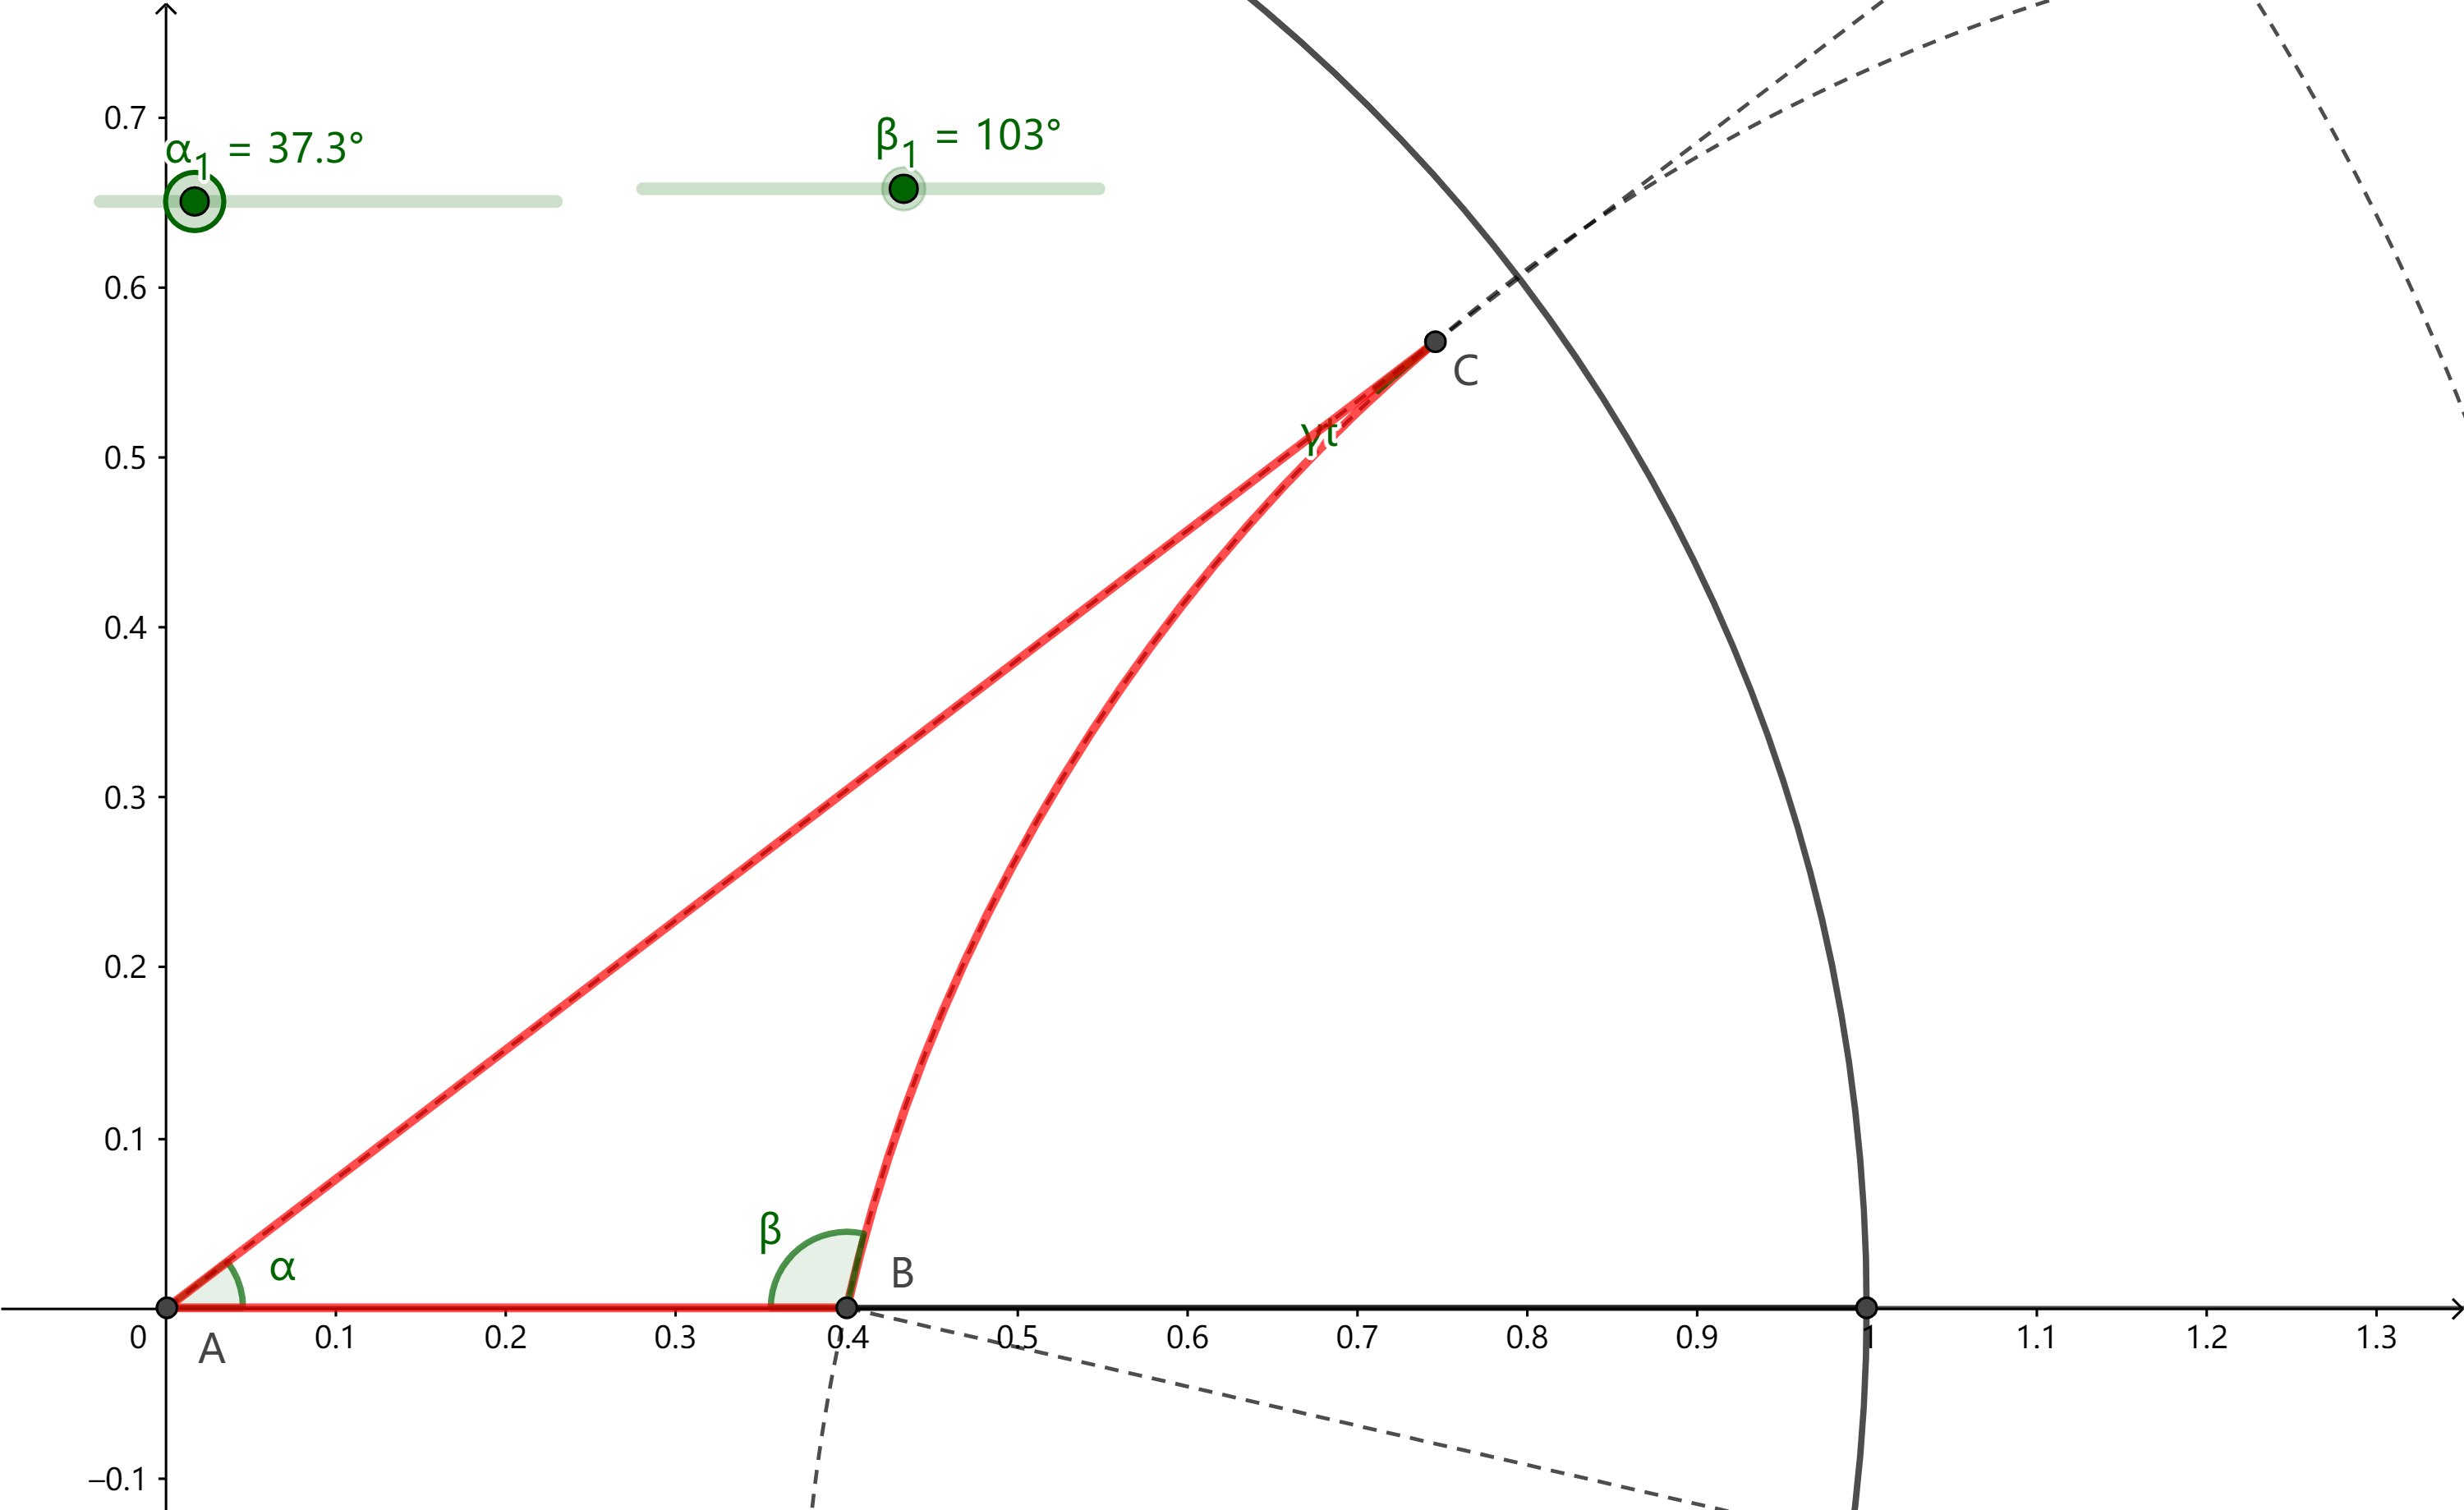
\includegraphics[width={0.9\linewidth}]{B1.png}
        \caption*{$t=0.4$}
    \end{minipage}
    \caption{$\gamma(t)$ changed\quad with\quad $t$}
    \label{gamma}
\end{figure}

\subsubsection{Nice pictures of hyperbolic triangle tiling}
\begin{figure}[ht]
    \centering
    \caption{Poincaré disk model of fundamental domain triangles}
    \label{Example}
    \begin{minipage}{0.49\linewidth}
        \centering
        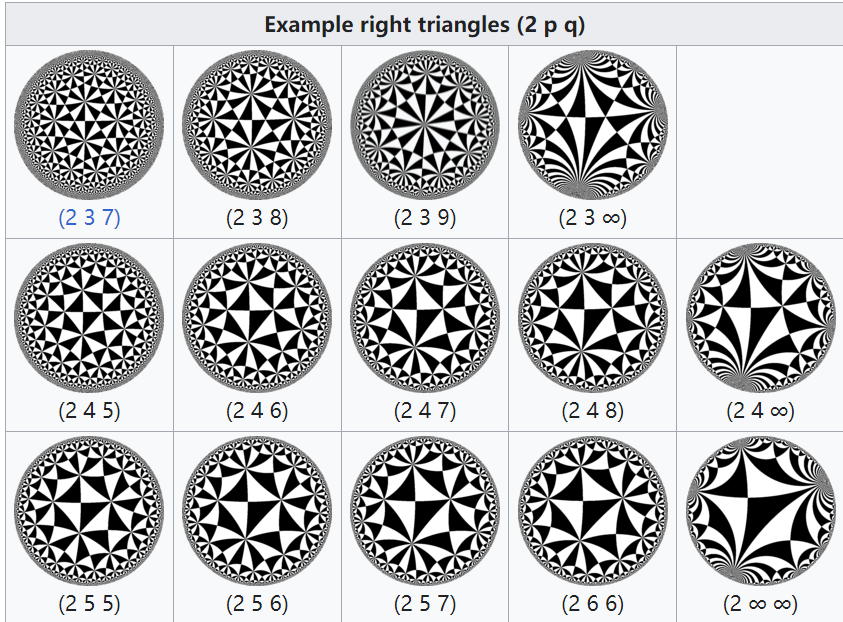
\includegraphics[width={0.9\linewidth}]{Example01.png}
    \end{minipage}
    \begin{minipage}{0.49\linewidth}
        \centering
        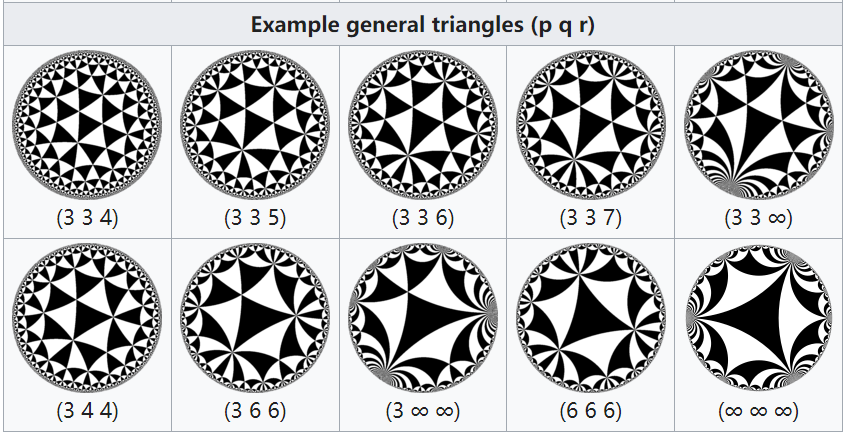
\includegraphics[width={0.9\linewidth}]{Example02.png}
    \end{minipage}
\end{figure}

\section{Finishing Remark}
This report is written mainly based on Wikipedia \cite{google}. Some details and ideas of forming general $(p, q, r)$ group are mainly learned in \cite{Tgt}. For a more precise and collective context for triangle group, \cite{tesselations} is highly recommended.

%==========reference=============
\newpage
\begin{thebibliography}{99}

    \bibitem{Tgt}
    Gross, J. L., \& Tucker, T. W. (2001). Topological graph theory. Courier Corporation.
    \bibitem{tesselations}
    Magnus, W. (1974). Noneuclidean tesselations and their groups. Academic Press.
    \bibitem{google}
    \url{https://en.wikipedia.org/wiki/Triangle\_group}
\end{thebibliography}
\end{document}